%% PeerJ Computer Science -- AI Application
%% Peer-review version: line numbering is enabled via the `lineno' option.
%% Camera-ready submissions should remove the `lineno' option.
%% The wlpeerj.cls class file is provided by PeerJ's LaTeX/Overleaf template.

\documentclass[fleqn,10pt,lineno]{wlpeerj}

% --- Fonts: T1 is needed for Turkish glyphs (ı, ğ, ç, ş) with the class's Times
% fonts. inputenc(utf8), amsmath, graphicx and xcolor are loaded by wlpeerj.cls.
\usepackage[T1]{fontenc}
\usepackage{float} % [H] placement for Figures 5/6 (avoids the LaTeX float-page vfill gap)
\usepackage{colortbl} % zebra-striping trial for Table 9 (\rowcolor)
\definecolor{tblstripe}{gray}{0.93}
\usepackage{url} % \url{} appears in the apalike bibliography (howpublished/notes)
% allow long reference URLs to break across lines (avoids margin overflow)
\Urlmuskip=0mu plus 1mu\relax
\makeatletter\g@addto@macro\UrlBreaks{\do\/\do\-\do\.\do\:\do\?\do\&\do\=\do\_}\makeatother

% Tighter table typesetting to save pages: less row/column padding.
\renewcommand{\arraystretch}{0.92}
\setlength{\tabcolsep}{4.5pt}

% Tighter float spacing: less air around and between figures/tables.
\setlength{\floatsep}{8pt plus 2pt minus 2pt}
\setlength{\textfloatsep}{10pt plus 2pt minus 3pt}
\setlength{\intextsep}{8pt plus 2pt minus 2pt}

% wlpeerj v1.2 removed \keywords; re-provide it and print it after \maketitle.
\makeatletter
\providecommand{\keywords}[1]{\gdef\@pjkw{#1}}
\newcommand{\printkeywords}{\ifdefined\@pjkw
  \par\smallskip\noindent{\color{color1}\sffamily\bfseries Keywords:\ }\@pjkw\par\medskip\fi}
\makeatother

\title{Learning-Assisted Exposure Assessment at Estate Scale: Constraint Recovery, Inventory Redundancy, and Engine Placement in Managed Enterprise Networks}

\author[1]{Ramazan Kocaoğlu}
\author[1]{Basma Bakırcı}

\affil[1]{Department of Computer Engineering, Ostim Technical University, Ankara, Turkey}

\corrauthor[1]{Ramazan Kocaoğlu}{ramazan.kocaoglu@ostimteknik.edu.tr}

\keywords{vulnerability assessment, network asset management, software inventory, sequence labelling, network security, network operations}

\begin{abstract}
Managed enterprise networks maintain an inventory of the software installed on every admitted endpoint, and that inventory is the natural input to per-asset vulnerability exposure assessment. Treated as independent queries the workload is intractable: a per-row scan of one estate examined here would exceed fourteen hours. This paper reports a measurement study of eight production estates comprising 2,525 endpoints and 336,918 live application records, and an assessment service designed around it. The inventory is a defective input in two ways no scanner can repair downstream: 46.7\% of live rows carry no version, so half an estate lies outside the addressable set before assessment begins, and the display strings that remain resolve poorly to standardised names---the canonical dictionary route yields a decidable product for 13.2\% of scannable rows---so normalisation rather than lookup dominates. What the inventory does offer is redundancy, at two levels: collapsing identical product--version pairs removes 88.5\% of the workload, and grouping the remaining items by product reduces repeated product-level preparation operations by a further 34.7\% while retaining a separate decision for every version. The redundancy is heavy-tailed, the largest one percent of items covering 10--52\% of rows while roughly half appear on a single endpoint. Constraint recovery from advisory prose, needed because only 574,995 of 1,128,919 affected-product records carry a machine-readable version bound, uses an 8.8M-parameter sequence tagger cached per advisory rather than per scan; operators are obtained by rule and product identity is never delegated to the model. What is reported below is whether the redesigned engine reproduces the reference implementation's verdicts under load, not whether either is correct; decision quality is evaluated in a companion study. Thread-level parallelism proved slower; moving candidate retrieval into memory removed the store from the per-item path; on a controlled 24-product workload the compiled concurrent engine was 9.6 times faster than the single-threaded reference implementation; and the tagger ran faster on a central processing unit (CPU) than on a graphics processing unit (GPU). A production inventory of 6,129 rows from 183 endpoints was reduced to 1,443 assessable items and scanned end to end in 368 seconds.
\end{abstract}

\begin{document}

\raggedbottom
\maketitle
\thispagestyle{empty}
\printkeywords

\section{Introduction}
\label{sec:intro}

Managed enterprise networks already record what an organisation runs. Admitting an endpoint requires identifying it, and enforcing posture policy requires enumerating what is installed on it, so the management platform---a network access control deployment in the estates studied here---maintains a continuous inventory of the software estate keyed by endpoint. That inventory is precisely the input a vulnerability exposure assessment needs, and precisely what most vulnerability tooling has to reconstruct by probing the network. But possessing it is not the same as being able to use it: the estates examined here export between six thousand and two hundred thousand application records each, the records report installer metadata rather than advisory nomenclature, and a substantial fraction omit the one field on which a verdict depends, so the obvious procedure---asking, for every record, whether a published vulnerability affects it---does not complete in an operational window.

A second incompleteness lies on the other side of the match. Only 574,995 of the 1,128,919 affected-product records in the corpus carry a machine-readable version bound; for the remainder the affected range exists only in the advisory's prose, or not at all. A service consulting structured fields alone is therefore blind to roughly half of the evidence, and the missing half cannot be recovered by better matching---it has to be extracted. A learned sequence tagger is used for that purpose, and its authority is deliberately bounded: it recovers version expressions from text and nothing else, comparison operators are obtained by rule, and product identity is never delegated to it.

This paper makes the resulting computation tractable and keeps it correct while it runs, approaching the problem as a network systems problem rather than a text processing one. What the verdict for a product--version pair should be is a question of decision quality treated here only as far as the systems argument requires: the semantics are stated, the assumptions made explicit, and the performance work shown not to have changed what the system decides. The questions answered are how an estate's worth of decisions is scheduled, how the missing constraints are recovered at scale, where the computation should be placed within a managed network, and what must hold for a multi-hour scan to survive contact with production. The starting observation is that estate inventories have structure, imposed by the way organisations provision endpoints, and that structure is exploitable.

\subsection{Contributions}

\begin{itemize}[noitemsep]
\item A measurement study of eight production enterprise software estates---2,525 endpoints and 336,918 live application records---reporting version coverage, two-level redundancy, fan-out concentration, per-endpoint density and the lexical transformations normalisation must survive. No comparable figures appear to have been reported, and they bound what any estate-scale assessment can achieve.
\item A coverage bound on the standard naming route, measured on the same estates: resolving display strings against the published CPE dictionary yields a decidable product for 2.6\% of product strings unassisted and 13.0\% under four increasingly generous normalisation tiers, of which 11.7\% also carry bounded applicability data. This establishes by measurement why an inventory-driven service cannot be built on dictionary lookup alone.
\item A learned constraint-recovery component that supplies the affected range where the corpus does not, with the scoping decisions that make it safe to deploy: extraction confined to version expressions, operators obtained by rule, identity decided outside the model, and outputs cached per advisory rather than per scan.
\item A two-level planning model separating estate-level deduplication from request-level sharing of version-invariant work, together with the correctness constraint that distinguishes them: preparation may be shared across the versions of a product, decisions may not.
\item A placement analysis in which client-side threading, a store on the per-item path, GPU inference and centralisation were each measured and each rejected---including a core-count sweep on a platform with one hardware thread per core, which locates where the parallel speed-up stops without confounding it with simultaneous multithreading, a per-item latency distribution, and a resource budget for the node.
\item An account of the transport and continuity properties such a service requires: a measured response-size failure, a measured request-granularity failure, a cache-key construction that survives code changes, and restart recovery verified on an interrupted job.
\end{itemize}

\section{Background and Related Work}
\label{sec:background}

\subsection{Asset Inventory as a Network Management Function}
Enterprise security frameworks place asset and software inventory first among controls, on the reasoning that no subsequent control can be applied to an asset that is not known \cite{cis,nistcsf}. In NAC-managed networks the inventory is a management artefact rather than a scanning result: admission and posture enforcement require endpoint identification, and installed-software enumeration follows from the same agent. This is an advantage over network-probing vulnerability assessment, which must infer installed software from exposed services and is well documented to be incomplete \cite{holm2011}.

The corresponding disadvantage is that the inventory speaks the vocabulary of installers rather than advisories. Standardised naming exists---Common Platform Enumeration provides a formal product identifier \cite{cpe} within the wider security automation protocol \cite{scap}---but the mapping from an agent-reported display string to a CPE name is exactly the step that is missing, and it is hard: CPE assignments are inconsistent with the records they describe \cite{sanguino2017}, automating the assignment is an active research problem \cite{hu2024,jiang2025vulcpe}, linking entities across naming systems remains open \cite{alfasi2024}, and software composition analysis tools disagree sharply on which components a project contains \cite{imtiaz2021,zhao2023}. What this literature does not report is how much of a real enterprise estate the mapping actually covers, its evidence being drawn from advisory records and open-source manifests rather than from the installed-application tables management platforms export. Section~\ref{sec:estate} quantifies the gap from that side, and Section~\ref{sec:cpe-route} measures the dictionary route's coverage directly.

\subsection{Vulnerability Assessment at Scale}
Network vulnerability analysis has largely been studied as a reachability and composition problem: given host-level weaknesses, derive multi-step attack paths \cite{sheyner2002,ou2011} and correlate the resulting alerts \cite{roschke2011}. That line of work assumes the per-host weakness set as input. The concern here is the production of that input at estate scale, which is upstream of attack-graph construction and, in the deployments observed here, the step that actually fails to complete.

Vulnerability intelligence itself is distributed across feeds with different guarantees---the CVE record set \cite{cvelist}, the enriched national database \cite{nvd}, an ecosystem-oriented open-source database \cite{osv}, exploitation observation and prediction \cite{kev,epss,jacobs2021}, severity scoring \cite{cvss}, and release support calendars \cite{endoflife}---and reconciling them is not mechanical. Only about 60\% of records match their standardised entries strictly, with the divergence growing over time \cite{dong2019}; affected-version data in particular is unreliable \cite{nguyen2013} and often recoverable only from prose \cite{glanz2015}; and severity scores are inconsistent across assessors and versions \cite{wunder2024,walkowski2026}. Feed ingestion is treated here as a background maintenance function (Section~\ref{sec:feeds}) whose network cost is reported rather than its epistemics.

The consequence for an operator is that exposure lists arrive long and unequally urgent, which is why prioritisation is a field of its own \cite{jiang2025survey} and why alert volume is a documented operational hazard \cite{tariq2025,jalalvand2025}. The concern here is upstream of prioritisation: producing the list at all, within a window that makes it actionable---a delay that is not theoretical, since patch application is already slowed by process and coordination factors before any tooling latency \cite{dissanayake2022}.

\subsection{Placement of Security Functions}
Where a network function executes is a design variable, and the arguments for moving computation toward the edge---latency, bandwidth, locality of sensitive data---are well rehearsed \cite{shi2016,mao2017,satya2017,bonomi2012}, as are the virtualisation and control-plane mechanisms that make placement flexible \cite{mijumbi2016,kreutz2015}. Vulnerability assessment has an unusually strong locality argument: a complete software inventory maps an organisation's attack surface, and transmitting it to an external service discloses in one document what an adversary would otherwise have to enumerate. The question is therefore not whether edge placement is desirable but whether it is feasible---an empirical question about the cost of the computation. Sections~\ref{sec:methodology} and~\ref{sec:results} answer it for the workload described here.

\subsection{Positioning}
Table~\ref{tab:positioning} places this work against the two families of system an operator would otherwise use. Network-probing scanners discover services rather than installed software, and are therefore blind to locally installed applications that expose no port---which, in the estates measured here, is most of them. Agent-reporting platforms know what is installed but report it in installer vocabulary and typically stop at inventory, leaving vulnerability correlation to a downstream service. It is that downstream service which is described here, designed for the case where the inventory already exists and the difficulty is its volume, its vocabulary, and its incompleteness.

% Table 1: Positioning against alternative sources of per-asset exposure.
\begin{table}[htbp]
\centering
\caption{Positioning against alternative sources of per-asset exposure.}
\label{tab:positioning}
\footnotesize
\begin{tabular}{l l l l}
\hline
Criterion & Network scanner & Agent inventory & This work \\
\hline
Discovery basis & exposed services & installed packages & given inventory \\
Installed-application discovery & partial & broad & broad \\
Assessable coverage & inferred from banner & version-dependent & version-dependent \\
Naming & service banner & installer string & normalised \\
Unit of work & host & row & reduced item \\
Version semantics & inferred & reported & adjudicated \\
Placement & network vantage & endpoint & in-network service \\
\hline
\end{tabular}
\end{table}


One row of Table~\ref{tab:positioning} deserves emphasis. An agent that enumerates installed packages discovers applications a network probe cannot see, so its discovery is broad; but discovery is not assessability. A record naming a product without naming its version supports no version comparison and therefore no verdict, and Section~\ref{sec:version-coverage} measures how large that gap is in practice: coverage claims for inventory-driven assessment are meaningful only when the versionless share is reported beside them.

\subsection{Relation to Earlier Work by the Authors}
An earlier version of this system was reported as a multi-model pipeline in which product relevance was decided by a parallel ensemble of language and entailment models. It has been replaced by the architecture described here, in which a single small sequence tagger recovers constraints from advisory prose and all adjudication is explicit. The decision-quality evidence motivating that replacement is the subject of a separate study; the present paper concerns the estate-scale and deployment questions, and treats the per-item decision procedure as given (Section~\ref{sec:pipeline}).

\section{The Estate-Scale Problem}
\label{sec:problem}

\subsection{Decision Semantics, in Brief}
The service takes as input a list of items, each an inventory row's product string and version with optional vendor and operating-system context, and returns for each item a verdict together with the per-advisory findings that support it. Two levels of vocabulary are therefore in play and are kept distinct throughout: an item carries one verdict, while a finding records what one advisory implies about that item, and an item's verdict summarises the findings beneath it.

For each inventory item the service emits one of four verdicts. \textbf{Threat} asserts that an advisory concerns the same product and that the installed version lies within an affected interval; \textbf{Safe} asserts that at least one of these is determinably false; \textbf{NotFound} asserts that no advisory record concerns the product at all; and \textbf{Uncertain} asserts that the available evidence determines none of the above. Findings are bucketed by the same three substantive outcomes, and where counts of findings are reported below the operator-facing wording is used---\emph{cleared} for a finding that establishes Safe, \emph{undetermined} for one that establishes Uncertain---because that is the wording the console and the API present. The two vocabularies name the same three outcomes at two levels of aggregation.

The third of these is load-bearing rather than decorative. Because the loss is asymmetric---a false threat produces an unnecessary quarantine and, repeated, trains operators to discount the channel \cite{tariq2025,jalalvand2025}---the engine does not emit Threat when product identity is not structurally confirmed. Declining to answer rather than answering wrongly is a long-standing formulation \cite{chow1970,elyaniv2010}; what differs here is that the abstention is not a threshold on a learned score, whose calibration in neural models is known to be poor \cite{guo2017}, but is taken on structural evidence---whether the applicability gates confirm identity and whether an interval is well formed. The consequence for scheduling is that an item which cannot be decided terminates quickly rather than escalating, and the estate-wide cost distribution is correspondingly less skewed than under a forced binary choice.

\subsection{Cost Model}
Let an estate export $R$ application rows drawn from $E$ endpoints. Write $U$ for the number of distinct scan items after identical rows are merged, and $G$ for the number of distinct products among them, so that
\begin{equation}
G \leq U \leq R,
\end{equation}
and define the two reduction ratios
\begin{equation}
\rho_{\text{item}} = \frac{R}{U}, \qquad \rho_{\text{group}} = \frac{U}{G}.
\end{equation}
$\rho_{\text{item}}$ measures how many endpoint records collapse onto one scan item; $\rho_{\text{group}}$ measures how many versions of a product coexist in the estate.

The per-item cost decomposes into a version-invariant part and a version-specific part. Retrieving candidate advisories for a product, loading their declared version boundaries, and extracting constraints from their descriptions all depend on the product and not on the installed version; only the interval comparison depends on the version. Writing $c_{\text{prep}}$ and $c_{\text{dec}}$ for the two, three scheduling policies give
\begin{align}
C_0 &= R\,(c_{\text{prep}} + c_{\text{dec}}) & \text{per row}, \\
C_1 &= U\,(c_{\text{prep}} + c_{\text{dec}}) & \text{per item}, \\
C_2 &= G\,c_{\text{prep}} + U\,c_{\text{dec}} & \text{per group}.
\end{align}
Because $c_{\text{dec}} \ll c_{\text{prep}}$---Section~\ref{sec:results} measures the ratio two ways---the achievable saving is governed almost entirely by $\rho_{\text{item}}$ and $\rho_{\text{group}}$, which are properties of the estate rather than of the scanner. Whether the model is worth building therefore depends on empirical values that were not available, and Section~\ref{sec:estate} obtains them.

A fourth cost regime matters more than any of these in steady operation. An estate is scanned repeatedly and changes only incrementally between scans. Writing $U_t$ for the item set at time $t$ and $\kappa$ for the per-item cost of a cache hit, a re-scan costs
\begin{equation}
C_\Delta = |U_t \setminus U_{t-1}|\,(c_{\text{prep}} + c_{\text{dec}}) + |U_t \cap U_{t-1}|\,\kappa,
\end{equation}
provided the cached verdicts remain valid---a condition that depends on the cache key rather than on elapsed time, which Section~\ref{sec:transport} makes precise. Since $\kappa$ is measured at roughly 12 ms against seconds for a cold item, steady-state cost is governed by the size of the change set rather than by the size of the estate; the concentration result of Section~\ref{sec:estate} predicts that change sets are small even when many endpoints are affected, because an upgrade rolled across a thousand machines introduces one item.

Cold-scan figures are reported throughout regardless, because the aggregate is governed by its slowest constituents rather than by the mean \cite{dean2013} and because they are what can be measured without a longitudinal deployment: the full cold scan happens once, at onboarding, and the recurring cost is $C_\Delta$.

\subsection{The Constraint That Bounds the Optimisation}
One constraint must be stated before the measurements, because it prevents the reduction from being taken further. Sharing $c_{\text{prep}}$ across the versions of a product is sound; merging the versions themselves is not. Two releases of the same product are affected by different advisory sets, so a scanner that collapses them returns a verdict correct for at most one---a correctness error whose surface form is an optimisation, easy to introduce and hard to notice: the merged scan is faster, the output well formed, and the error visible only against ground truth for the discarded version. The planner of Section~\ref{sec:planning} keeps the two operations structurally distinct for this reason.

\section{Estate Structure: A Measurement Study}
\label{sec:estate}

\subsection{Data and Method}
Software inventory exports were analysed from eight production enterprise deployments of a commercial NAC platform, obtained during integration projects and used here with the operators' consent. Each is a dump of the platform's installed-application table, carrying an endpoint identifier, a product display name, a version string, a vendor string, an architecture marker and a deletion flag. A ninth export is excluded: produced against a dropped database connection, it contains a serialised exception in place of every value, and the exclusion is recorded in the analysis script's own output rather than only here.

The reduction reproduces the deployed exporter. Rows flagged as deleted are discarded, as are rows without a product name; rows without a version are discarded as unscannable, and counted, because a verdict is a version comparison and a row lacking one can only abstain. Remaining rows are merged on (product name, version) after whitespace and case normalisation. One deviation should be noted: the exporter's merge key additionally includes the endpoint's operating-system family, because the same display name on different platforms is not the same installation, and these exports carry no operating-system join. Since the omitted component can only split groups, the reduction and fan-out figures reported below are upper bounds on what the deployed exporter achieves.

Two aggregate properties precede the reduction and bound what it operates on. The eight exports contain 394,316 rows of which 57,398 (14.6\%) are flagged deleted: roughly one row in seven describes an installation that is no longer present, and a consumer that ignores the flag inflates its workload accordingly while reporting exposure for software that is not installed. And the estates carry 133.4 live application rows per endpoint on average, falling to 71.1 scannable rows and 8.1 distinct scan items per endpoint after reduction---the per-endpoint form of the ratios below, and the figures to use when sizing an assessment against an endpoint count rather than a row count.

Both analyses are implemented as standalone scripts released with this paper, so the figures can be regenerated from the exports.

\subsection{Version Coverage}
\label{sec:version-coverage}
The first result concerns whether the inventory is usable at all. A verdict is a version comparison, so a row without a version cannot produce one; and the comparison itself presumes an ordering that enterprise software does not uniformly provide, since adherence to semantic versioning \cite{semver} is partial even in curated package ecosystems \cite{li2023golang,venturini2023} and the affected range must often be recovered from the advisory rather than read from a field \cite{bao2022}. Table~\ref{tab:version-coverage} reports, for each estate, the number of live application rows---not deleted, carrying a product name---and the proportion of them that carry no version string.

% Table 2: Version coverage of live application rows.
\begin{table}[htbp]
\centering
\caption{Version coverage of live application rows. A row without a version cannot produce a verdict.}
\label{tab:version-coverage}
\footnotesize
\begin{tabular}{l r r r}
\hline
Estate & Endpoints & Live rows & No version \\
\hline
E1 & 176 & 15,006 & 38.2\% \\
E3 & 957 & 198,835 & 59.1\% \\
E4 & 88 & 5,979 & 0.7\% \\
E5 & 183 & 14,125 & 7.1\% \\
E6 & 526 & 52,583 & 33.9\% \\
E7 & 79 & 6,447 & 16.0\% \\
E8 & 361 & 37,336 & 37.6\% \\
E9 & 155 & 6,607 & 4.5\% \\
\hline
Pooled & 2,525 & 336,918 & 46.7\% \\
\hline
\end{tabular}
\end{table}


Across the pooled estates, 46.7\% of live application rows carry no version. The spread is the more informative part of the result: from 0.7\% in E4 to 59.1\% in E3, a range too wide to be a property of the software population. The exports carry no field recording how each agent was configured, so the cause cannot be established from this data; the missingness is likely attributable to agent configuration and platform-version differences across deployments, and we report the association rather than a demonstrated cause. Two practical consequences follow, neither depending on which explanation is correct: a scanner's coverage figure is not comparable across deployments unless the versionless share is reported alongside it, since half of one estate is simply outside the addressable set; and the highest-value intervention for an operator of an estate like E3 is not a better scanner but an inventory that records versions---an upstream change in the access control platform's own collection. These rows are treated as out of scope rather than as failures and are excluded from every subsequent count, so that the redundancy figures below describe the scannable workload.

\subsection{Two Levels of Redundancy}
That large collections of machine-installed files repeat heavily is not itself new---file-system studies have measured both the content distribution across enterprise desktops \cite{douceur1999} and the deduplication ratios achievable over them \cite{meyer2012}. What appears not to have been reported is the equivalent structure in the application inventory a management platform exports, which is the object a vulnerability service actually consumes. Table~\ref{tab:redundancy} reports the reduction structure over the scannable rows.

% Table 3: Two-level redundancy in production estates.
\begin{table}[htbp]
\centering
\caption{Two-level redundancy in production estates. $R$ is scannable rows, $U$ distinct scan items, $G$ distinct products. The pooled row sums each column over the eight estates rather than de-duplicating across them, because each estate is scanned as a separate workload: a product present in five estates is five preparation units, not one.}
\label{tab:redundancy}
\footnotesize
\begin{tabular}{l r r r r r r}
\hline
Estate & $R$ & $U$ & $G$ & $\rho_{\text{item}}$ & $\rho_{\text{group}}$ & Reduction \\
\hline
E1 & 9,271 & 1,510 & 1,011 & 6.1 & 1.49 & 83.7\% \\
E3 & 81,368 & 4,741 & 2,946 & 17.2 & 1.61 & 94.2\% \\
E4 & 5,940 & 721 & 432 & 8.2 & 1.67 & 87.9\% \\
E5 & 13,120 & 2,377 & 1,524 & 5.5 & 1.56 & 81.9\% \\
E6 & 34,779 & 4,632 & 3,123 & 7.5 & 1.48 & 86.7\% \\
E7 & 5,417 & 1,629 & 1,200 & 3.3 & 1.36 & 69.9\% \\
E8 & 23,282 & 3,316 & 2,162 & 7.0 & 1.53 & 85.8\% \\
E9 & 6,311 & 1,635 & 1,026 & 3.9 & 1.59 & 74.1\% \\
\hline
Pooled & 179,488 & 20,561 & 13,424 & 8.7 & 1.53 & 88.5\% \\
\hline
\end{tabular}
\end{table}


Merging identical product--version pairs removes 88.5\% of the pooled workload; no estate falls below 69.9\%. The second level is smaller but not negligible: 1.53 versions per product on average, so that grouping the remaining items by product reduces repeated product-level preparation operations by a further 34.7\%, while retaining a separate decision for every version. The distinction matters and is not pedantry. The 34.7\% applies to preparation---candidate retrieval, boundary loading, constraint extraction---and to nothing else; the number of decisions is unchanged at $U$, because two versions of a product are two verdicts however their preparation was obtained. A reduction claimed over decisions rather than over preparation would be the correctness error Section~\ref{sec:problem} describes, expressed as a performance figure. Estates differ substantially in the first ratio---E3 at 17.2 against E7 at 3.3---and the difference is interpretable. E3 is a large, centrally imaged estate in which most endpoints receive an identical software build; E7 is small and heterogeneous. Redundancy is therefore a function of provisioning discipline, and the estates that are largest are, conveniently, the ones where reduction helps most.

The second ratio varies far less, between 1.36 and 1.67, which suggests it reflects update-rollout dynamics---a product is mid-migration across the estate---rather than local policy. Its stability matters for design: a scanner can rely on group sharing being worth implementing without tuning for the deployment.

\subsection{Version Spread Within Products}
The second ratio is an average over a population that is itself skewed, and the skew is what makes the never-merge-versions constraint operationally consequential rather than merely formally correct. Table~\ref{tab:version-spread} reports how many products appear at more than one version and how far the spread goes.

% Table 4: Version spread within products.
\begin{table}[htbp]
\centering
\caption{Version spread. Products present at several versions simultaneously, and the widest spread observed in each estate.}
\label{tab:version-spread}
\footnotesize
\begin{tabular}{l r r r}
\hline
Estate & Products $G$ & Multi-version & Widest spread \\
\hline
E1 & 1,011 & 166 (16.4\%) & 31 versions \\
E3 & 2,946 & 486 (16.5\%) & 69 versions \\
E4 & 432 & 121 (28.0\%) & 16 versions \\
E5 & 1,524 & 294 (19.3\%) & 69 versions \\
E6 & 3,123 & 566 (18.1\%) & 70 versions \\
E7 & 1,200 & 169 (14.1\%) & 27 versions \\
E8 & 2,162 & 430 (19.9\%) & 77 versions \\
E9 & 1,026 & 201 (19.6\%) & 53 versions \\
\hline
\end{tabular}
\end{table}


Between 14\% and 28\% of products are present at more than one version at the moment of export, and the widest spreads run to seventy-odd distinct versions of a single product coexisting in one estate. These are the products in the middle of a rollout, or the ones whose updates are not centrally managed at all.

The consequence is that merging versions is not a rare corner case whose cost could be tolerated. A scanner that collapsed each product to one version would be answering for one release and reporting the answer for up to seventy others, and it would do so for a fifth of every estate's products---exactly the products in a heterogeneous patch state and therefore the ones whose exposure differs most across endpoints. That such heterogeneity is the norm rather than the exception is well documented: patch adoption is slow and uneven across a population \cite{li2017}, and shared code means a single flaw reaches machines through several independently versioned products \cite{nappa2015}. The correctness constraint of Section~\ref{sec:problem} is thus binding on a large and security-relevant subset of the workload, and the modest average of 1.53 conceals it.

\subsection{The Redundancy Is Concentrated}
An aggregate ratio conceals whether the redundancy is spread evenly or concentrated in a head, and the two imply different caching strategies. The distinction is the same one that governs web cache design, where a Zipf-like popularity distribution bounds achievable hit rates and makes the tail, not the head, the limiting factor \cite{breslau1999}. Table~\ref{tab:fanout} reports the distribution of endpoint fan-out per item.

% Table 5: Fan-out distribution.
\begin{table}[htbp]
\centering
\caption{Fan-out distribution: how many endpoints share a scan item. Head shares give the proportion of scannable rows covered by the largest items; singletons appear on exactly one endpoint.}
\label{tab:fanout}
\footnotesize
\begin{tabular}{l r r r r r r r r}
\hline
Estate & p50 & p90 & p99 & max & Top 1\% & Top 5\% & Top 10\% & Singletons \\
\hline
E1 & 1 & 10 & 131 & 363 & 27.2\% & 60.0\% & 70.8\% & 56.8\% \\
E3 & 1 & 8 & 714 & 1,838 & 51.9\% & 85.8\% & 90.3\% & 55.3\% \\
E4 & 2 & 30 & 75 & 150 & 10.3\% & 43.5\% & 69.7\% & 39.1\% \\
E5 & 1 & 8 & 113 & 321 & 24.2\% & 58.2\% & 69.1\% & 56.4\% \\
E6 & 2 & 9 & 136 & 858 & 43.5\% & 67.2\% & 75.6\% & 48.8\% \\
E7 & 2 & 5 & 35 & 65 & 14.1\% & 33.5\% & 43.1\% & 40.0\% \\
E8 & 1 & 9 & 122 & 678 & 41.3\% & 66.7\% & 76.5\% & 60.3\% \\
E9 & 2 & 6 & 53 & 148 & 20.2\% & 46.8\% & 57.2\% & 37.6\% \\
\hline
\end{tabular}
\end{table}


The distribution is extreme. The median item appears on one or two endpoints, while the largest appears on 1,838 in E3---an estate of 957 endpoints, so the item is installed more than once per machine, which is what a suite of per-language proofing components looks like in an inventory. The top one percent of items covers between 10.3\% and 51.9\% of all rows, and between 37.6\% and 60.3\% of items appear on exactly one endpoint.

\begin{figure}[!htbp]
\centering
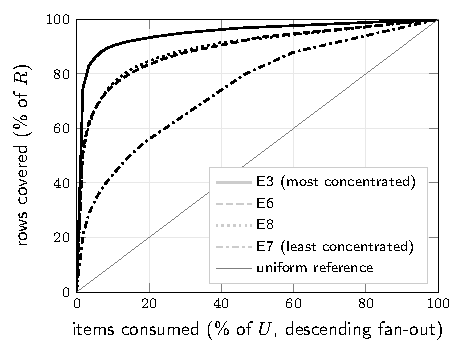
\includegraphics[width=0.55\linewidth,height=0.4\textheight,keepaspectratio]{figures/Figure_1}
\caption{Fan-out concentration. In every estate a small head of items covers most rows, but the curves flatten well below 100\%, and the residual is the singleton tail that no cache can warm.}
\label{fig:fanout}
\end{figure}

Figure~\ref{fig:fanout} plots the full concentration curve for four estates spanning the observed range. Each curve gives the cumulative share of scannable rows covered as items are consumed in descending order of fan-out; the diagonal is the reference a perfectly uniform estate would follow. Every curve rises steeply and then flattens, and the shape rather than the endpoint is what matters. In E3 the first 1.7\% of items already covers 74.5\% of rows; thereafter the curve gains roughly ten percentage points over the remaining 98\% of the item population. Even in E7, the least concentrated estate, the first fifth of items covers over half the rows. The estates differ in how steep the head is, not in whether one exists.

Two design consequences follow, and they pull in opposite directions. The head justifies caching persistently rather than within a run: a small number of items accounts for a large share of the work in every estate, and those items---the corporate browser build, the office suite, the endpoint agent---are also the ones most likely to recur in the next scan and in a different estate, whereas a cache scoped to a single scan captures only the intra-run duplicates the planner would remove anyway (Section~\ref{sec:transport}). The tail bounds what caching can do: because roughly half of all items are singletons, half the item population is cold on every run however large the cache, so any projection assuming a uniform warm cache is wrong, and none is made here.

\subsection{What Normalisation Must Survive}
The final estate property concerns the product strings themselves. Table~\ref{tab:lexical} reports the prevalence of lexical features that must be removed or tolerated before an inventory name can be compared with an advisory product name, computed per name rather than per row so that a single widely deployed application does not dominate. The denominator is the 13,424 product strings summed over the eight estates, consistent with the pooled column of Table~\ref{tab:redundancy}; de-duplicated across estates the same population comprises 7,604 distinct strings, and the two are distinguished because a summed count read as a distinct one would overstate the diversity of the name population.

% Table 6: Lexical features of inventory product strings.
\begin{table}[htbp]
\centering
\caption{Lexical features of inventory product strings, over the 13,424 product strings summed across the eight estates (7,604 distinct after de-duplication across estates). Classes are not mutually exclusive.}
\label{tab:lexical}
\footnotesize
\begin{tabular}{l l r}
\hline
Feature & Example fragment & Share \\
\hline
Vendor prefix & Microsoft\ldots, Google\ldots & 55.4\% \\
Embedded version & \ldots 14.40.33810 & 46.2\% \\
Architecture marker & (x64), 32-bit & 40.8\% \\
Year designator & \ldots 2016 & 24.7\% \\
Packaging vocabulary & Redistributable, Click-to-Run & 21.8\% \\
Non-ASCII characters & Çalışma Zamanı & 5.9\% \\
Locale qualifier & MUI (Turkish), Deutsch & 5.0\% \\
Edition qualifier & Professional, Enterprise & 3.3\% \\
\hline
\end{tabular}
\end{table}


The three most prevalent classes each affect roughly half the name population, which settles a design question that might otherwise be argued from taste: normalisation is not a preprocessing convenience but the dominant lexical operation, and a matcher assuming advisory-like input will fail on most of the estate. The embedded-version class is the most treacherous, since a name such as \texttt{Microsoft Visual C++ 2015-2022 Redistributable (x86) - 14.40.33810} carries a version that need not equal the version field, while a normaliser stripping numerals indiscriminately destroys product identity along with them. The mismatch appears directly in the production inventory of Section~\ref{sec:results}, where a widely deployed redistributable has a name ending in \texttt{14.44} and a version field reading \texttt{14.44.35211.0}.

The localisation classes are individually small---5.9\% non-ASCII, 5.0\% explicit locale qualifiers---but they concentrate in exactly the head items identified above, because office suites ship per-language components. In E3 the eight most widely installed items are all localised proofing or interface components of one office suite, each present on 919 endpoints. A matcher that mishandles locale qualifiers therefore mishandles a disproportionate share of the estate's rows even though it mishandles a small share of its names.

\subsection{What the Standard Naming Route Achieves}
\label{sec:cpe-route}
The preceding subsection argues indirectly, from lexical prevalence, that normalisation is unavoidable. The direct question is how far the standard procedure gets without it. Every inventory-driven assessment tool implements essentially one pipeline---resolve the display string to a canonical product identifier, retrieve advisories whose applicability rows name that identifier, compare versions---and the natural identifier is the Common Platform Enumeration name \cite{cpe}, resolved through the published CPE dictionary. Measuring that pipeline gives a baseline for the approach rather than for any vendor's implementation of it, which is the comparison this work can make honestly: a network-probing scanner is excluded by construction, since it cannot observe a locally installed application at all.

The measurement resolves each estate's scannable product strings against the non-deprecated application entries of the dictionary in four cumulative tiers: case folding and punctuation collapse, as an unassisted lookup performs; then removal of architecture markers and packaging vocabulary; then locale, edition and year qualifiers; then embedded version numerals. The later tiers exceed what a CPE-based scanner would normally attempt---the fourth is actively unsafe, destroying identity for products whose numeral is part of the name---so a string resolving under none of them has not merely been matched carelessly. Because resolution alone does not suffice for a verdict, a second stage checks whether the corpus carries applicability rows for the resolved product and whether those rows carry a version bound.

% Table 7: The CPE-dictionary route on the eight estates.
\begin{table}[htbp]
\centering
\caption{The CPE-dictionary route on the eight estates: share of scannable product strings, and of the rows they cover, that survive each stage. Resolution tiers are cumulative.}
\label{tab:cpe-route}
\footnotesize
\begin{tabular}{l r r}
\hline
Stage & By name & By row \\
\hline
\multicolumn{3}{l}{\textit{Stage 1: resolution to a dictionary entry}} \\
Case and punctuation only & 2.6\% & 8.1\% \\
\quad + architecture, packaging & 2.9\% & 8.8\% \\
\quad + locale, edition, year & 4.9\% & 10.5\% \\
\quad + embedded version stripped & 13.0\% & 16.2\% \\
\multicolumn{3}{l}{\textit{Stage 2: decidable applicability}} \\
Resolved and version-bounded & 11.7\% & 13.2\% \\
\hline
\end{tabular}
\end{table}


The result bounds the approach rather than tuning it. An unassisted dictionary lookup resolves 2.6\% of the estates' product strings; the most generous normalisation this measurement permits raises that to 13.0\%, and requiring that the resolved product also carry a bounded applicability row leaves 11.7\%. Weighted by rows the figures are higher---8.1\%, 16.2\% and 13.2\% respectively---because the head items of an estate are widely deployed commercial applications whose naming the dictionary serves best, which is the same concentration effect Section~\ref{sec:estate} measures, seen from the naming side.

The obvious objection was checked rather than assumed. The dictionary divides its entries into applications, operating systems and hardware, and the measurement admits only applications; estates also carry operating-system update packages and drivers, which would then count as unresolvable through no fault of the lookup. Repeating the measurement with operating-system entries admitted, and again with hardware entries as well, leaves the row-weighted figures untouched at 16.2\% in all three cases and raises name-weighted resolution only from 13.0\% to 13.1\% and then 13.2\%---despite the dictionary growing from 43,706 keys to 138,158. Tripling the dictionary leaves estate coverage essentially unchanged, so the bound is not an artefact of which part of it was consulted.

The shape of the gain across tiers is itself informative. Architecture and packaging vocabulary add 0.3 percentage points and locale, edition and year qualifiers a further 2.0; the large step comes from stripping embedded version numerals, which alone accounts for more than half of what the four tiers achieve. That ordering is inconvenient, because numeral-stripping is precisely the tier that cannot be applied safely in general. Nor is the residue an exotic tail: the largest unresolvable strings by row count are ordinary corporate software---an endpoint security agent on 2,952 rows, an office suite edition on 2,544, a browser runtime component on 2,281, a vendor update tool on 2,058---which are the head items whose verdicts matter most.

Two things follow. The standard route leaves roughly seven-eighths of an enterprise estate undecidable, which is why this work treats normalisation and full-text retrieval as the primary matching path and the dictionary as one signal among several rather than as the index. And the measurement establishes what that route cannot do, not that the approach described here decides the remainder correctly; decision quality on the residual belongs to the companion study, which is why this is reported as a coverage bound and not as an accuracy comparison.

\subsection{Summary of Implications}
The measurements support four design commitments, each of which is realised in the system described next:
\begin{enumerate}[noitemsep]
\item \textbf{Reduce before scheduling.} With $\rho_{\text{item}} = 8.7$ pooled, the reduction is worth more than any subsequent scheduling improvement.
\item \textbf{Share preparation, not decisions.} With $\rho_{\text{group}} = 1.53$, group sharing is worth implementing everywhere, and the correctness constraint of Section~\ref{sec:problem} makes the distinction mandatory.
\item \textbf{Cache across scans, not within them.} The head is stable and recurring; the intra-run duplicates are already removed by reduction.
\item \textbf{Budget for a cold tail.} Roughly half of all items are singletons, so a warm-cache projection describes no real estate.
\end{enumerate}

\section{Service Architecture}
\label{sec:architecture}
The service is deployed as three processes plus a relational store, co-located with the NAC platform. Figure~\ref{fig:deploy} shows the arrangement.

\begin{figure}[!htbp]
\centering
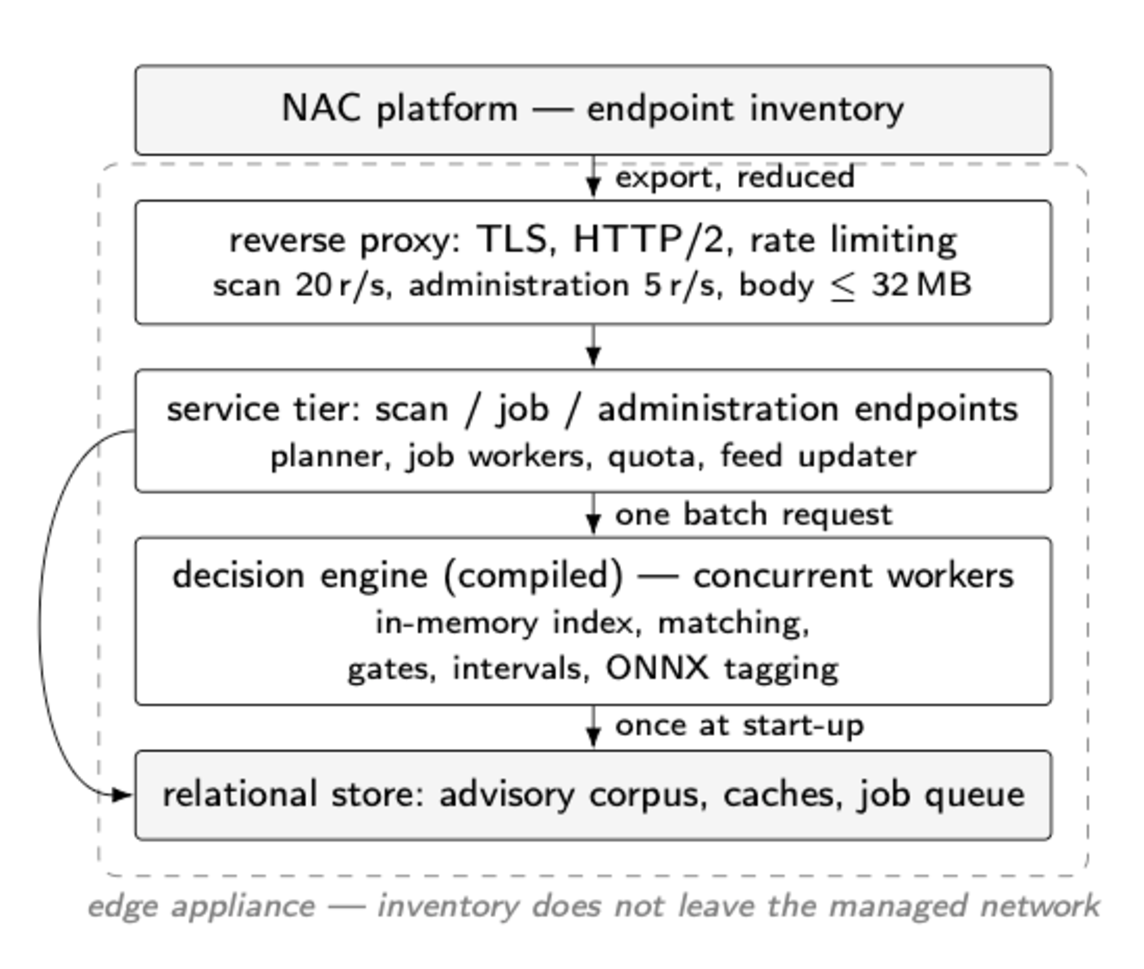
\includegraphics[width=0.7\linewidth,height=0.4\textheight,keepaspectratio]{figures/Figure_2}
\caption{Deployment. The inventory is reduced where it is held, submitted once, and adjudicated inside the managed network.}
\label{fig:deploy}
\end{figure}

The division of responsibility follows the location of the data. Everything that touches the corpus---candidate retrieval, version boundaries, applicability data, cached extractions, matching, gating, ranking---executes in the compiled engine alongside its connection pool, while the service tier owns request handling, authentication, quota, planning, the job queue, result caching, and feed maintenance. Placing the boundary anywhere inside the data access path was considered and rejected; Section~\ref{sec:results} gives the measurement that decided it.

Two dependencies degrade differently, and the difference is deliberate. Losing the engine stops scanning: the endpoints answer with a service-unavailable status and the caller retries, rather than quietly handing the work to the reference implementation---a fallback would put two decision implementations in production at once, with any drift surfacing as inconsistent verdicts and nothing in the response to indicate which path produced them. Losing the model runtime does not stop scanning: the engine proceeds from the extractions it already holds and names the advisories it could not process, so the answer arrives with its gaps declared. The first dependency governs whether a verdict is trustworthy, the second how much of the corpus it covers---an incomplete answer that says so is useful, whereas an unattributable one is not.

Integration with the access control platform is server-to-server, so no API credential reaches a browser; uploading an inventory and starting a scan are separate operations, so loading an estate does not commit an operator to the cost of scanning it.

\subsection{The Assessment Pipeline and Its Learned Component}
\label{sec:pipeline}
The per-item decision procedure is treated as given here and described only to the depth the systems argument requires; its learned component is stated in full, because what that component is permitted to decide bounds how much of the corpus can be assessed at all. The engine takes a product string, a version and optional vendor and operating-system context, and returns one of the four verdicts of Section~\ref{sec:problem} with the findings supporting it, a remediation proposal, and separately carried exploitation and severity signals. The components exercised in this paper are the normalised-name index, full-text retrieval over advisory descriptions, the applicability gates, the interval comparison and the sequence tagger; nothing else in the platform participates in a verdict. Whether the compiled and interpreted implementations agree is answered in Section~\ref{sec:verdict-preservation}, since the performance work would otherwise be unfalsifiable; whether the verdicts are correct is not evaluated here---precision, recall and abstention calibration belong to the companion study---and no claim in this paper depends on them being so.

\begin{figure}[!htb]
\centering
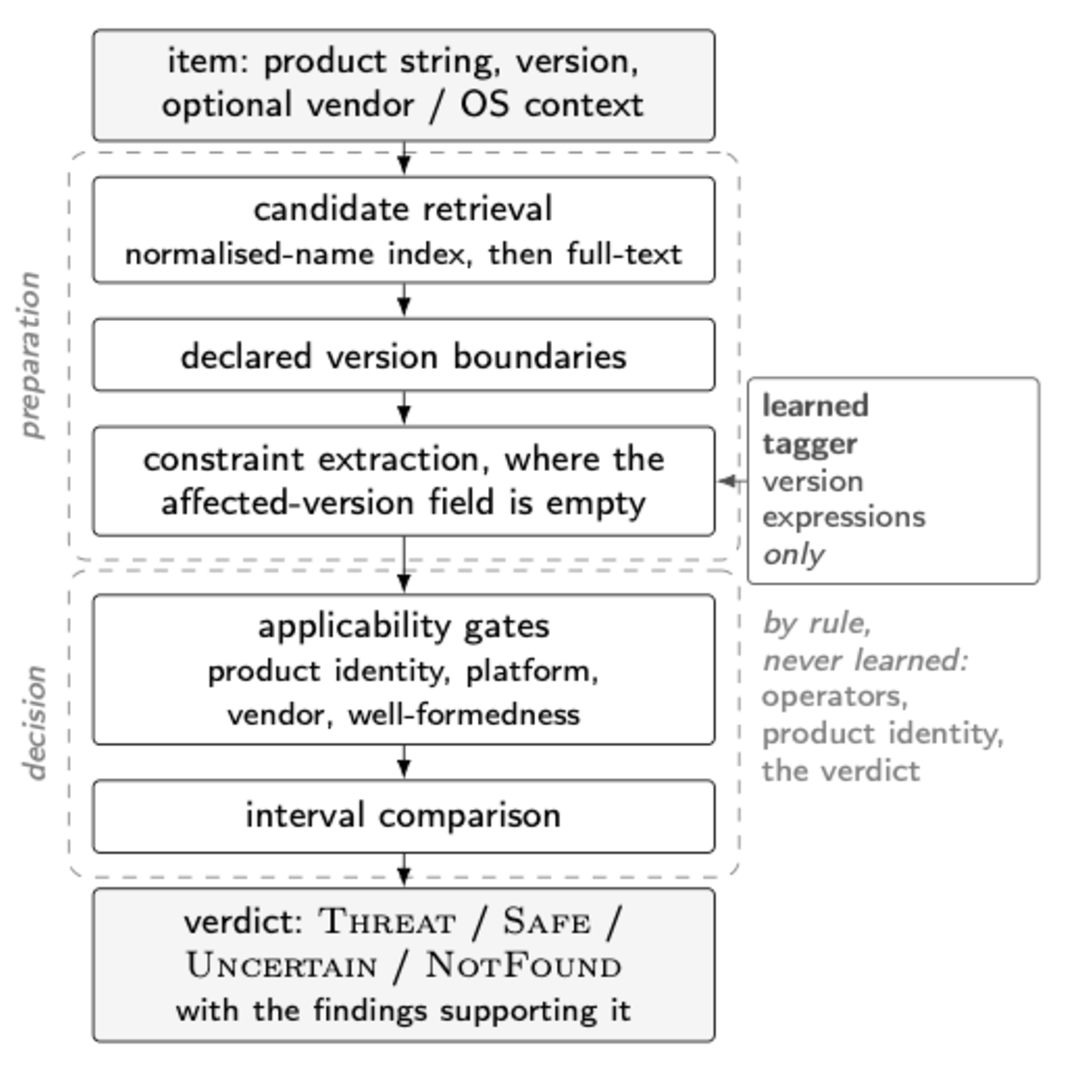
\includegraphics[width=0.7\linewidth,height=0.4\textheight,keepaspectratio]{figures/Figure_3}
\caption{The per-item decision procedure and the boundary of the learned component's authority. Preparation depends on the product alone and is executed once per product group; decision depends on the version and is executed once per version. The tagger contributes a constraint to one preparation stage and is consulted only after product identity has been settled structurally; comparison operators and verdicts are never delegated to it.}
\label{fig:pipeline}
\end{figure}

Figure~\ref{fig:pipeline} shows the two phases executed per submitted group. Preparation depends on the product alone; decision is repeated for each of its versions. The split is what the planner of Section~\ref{sec:planning} exploits, and the reason the learned component's position within it matters.

\paragraph{Why a learned component is required.}
Roughly half of all affected-product records carry no machine-readable version bound: 574,995 of 1,128,919 in the corpus. For those records the affected range is stated, if at all, in the advisory's prose, in forms that vary by numbering authority and by product family. No amount of improvement in name matching recovers them, because the deficiency is not in the match but in the field being matched against. Either the range is extracted from text or half the corpus is unusable. Extraction is performed by a bidirectional recurrent tagger with a conditional random field output layer and a character-level sub-encoder, 8.8M parameters in total. The character sub-encoder is not incidental: version strings such as \texttt{9.0.90}, \texttt{8u151} or \texttt{7.4.3.4726} do not occur in any vocabulary and cannot be represented by word-level embeddings alone.

\paragraph{What the component is not permitted to decide.}
Three boundaries are drawn deliberately, and each removes a class of error a more ambitious use of the model would introduce. Comparison operators are obtained by explicit rule: the relational vocabulary is a small closed class with unambiguous surface forms, and a model that occasionally inverts one produces an inverted verdict from an otherwise correct extraction---an error invisible in aggregate extraction accuracy and fatal in a single decision. Product identity is never delegated: whether an advisory concerns the installed product is settled by the applicability gates on structural evidence, and the tagger is consulted only after that question is closed, because a confident interval computed over a misidentified product is a well-formed and entirely wrong answer. And the model does not emit verdicts; its output is a constraint, adjudicated by the same interval logic that handles structured bounds, which take precedence where both exist.

\paragraph{Deployment properties.}
Two properties matter for the rest of the paper and are measured in Section~\ref{sec:results}. Extraction depends on the advisory text and not on the queried version, so results are cached per advisory rather than per scan; because advisories are estate-independent, that cache is warm across products, across scans and across networks. And inference runs on CPU, faster than on the GPU reference at this parameter count, which removes the accelerator from the deployment requirement.

\paragraph{Corpus defects are handled in the engine.}
One numbering authority's records place the operating-system build in which a patch shipped where the product's upper version bound belongs, a pattern present in 90,570 affected-product records; a well-formed comparison against such a bound is a comparison between two numbering systems. Together with a platform applicability class, handling these two removed 882 findings from the 1,443-item production inventory used in Section~\ref{sec:results} while leaving every cleared and not-found item unchanged. The effect is reported here because it bears on the workload---findings removed are findings not transported or paginated---while its security significance is left to the separate decision-quality study.

\section{Redundancy-Aware Planning}
\label{sec:planning}
Planning happens at two places, corresponding to the two levels of redundancy measured in Section~\ref{sec:estate}. Figure~\ref{fig:planning} shows the two together with the constraint that separates them.

\begin{figure}[!htbp]
\centering
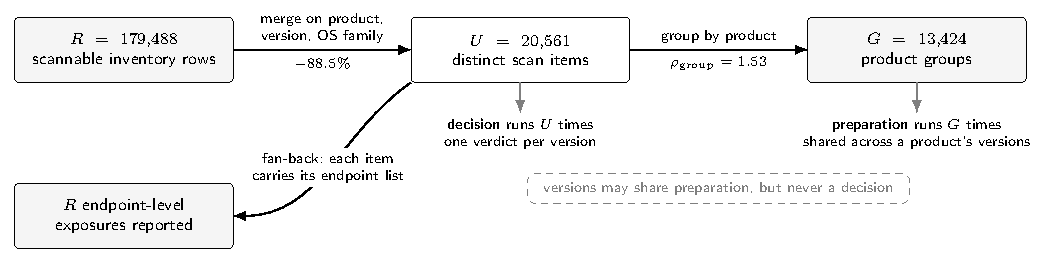
\includegraphics[width=0.85\linewidth,height=0.4\textheight,keepaspectratio]{figures/Figure_4}
\caption{Two-level redundancy-aware planning, with the pooled figures of Table~\ref{tab:redundancy}. Merging identical product--version pairs removes 88.5\% of the rows; grouping the survivors by product shares the version-invariant preparation without merging the versions themselves, so the number of decisions stays at $U$. Because each item retains the endpoints that contributed to it, the reduction is invisible in the report: the scan computes $U$ verdicts and the console still reports exposure for all $R$ rows.}
\label{fig:planning}
\end{figure}

\subsection{Estate-Level Reduction and Fan-Back}
The first reduction is performed where the inventory lives. An exporter reads the NAC installed-application table and emits scan items merged on product, version, and operating-system family, carrying with each item the list of endpoints that contributed to it.

The choice of merge key is where the design decisions are. Version is included, for the correctness reason of Section~\ref{sec:problem}. Operating-system family is included, because platform applicability changes the verdict: the same display name on Windows and macOS is not the same installation. Vendor is deliberately excluded, because agents populate it inconsistently---some rows for a product carry a vendor string and others do not---and including an inconsistently populated field in a merge key splits one product into several groups. Instead the most frequent non-empty vendor within a group is adopted for the whole group, which recovers the field's information without letting its absence fragment the key.

Because each item retains its endpoint list, one verdict propagates back to every endpoint that contributed. The scan computes $U$ decisions and the console reports $R$ endpoint-level exposures. This fan-back is what makes the reduction acceptable to operators: the reduction is an implementation property, and the reporting granularity is unchanged.

\subsection{Request-Level Grouping}
The second reduction is performed inside the service. A planner converts the submitted item list into groups sharing the version-invariant work, and maintains two distinct mappings: an assignment from each submitted position to the unique item that will answer it, and a grouping of unique items by product. The first handles exact duplicates that survived estate-level reduction---they occur whenever a caller submits a raw list---and the second handles the different versions of one product.

The response preserves the submitted order and length. A caller receives exactly as many results as it sent, in the order it sent them, with copied results marked as such so the distinction between a computed and a propagated verdict remains visible.

\subsection{Closing the Loop with the Access Control Platform}
Reduction and fan-back turn the assessment into a function the NAC platform can call rather than a report an analyst reads. Three properties make that integration workable, and each follows from a design decision above. The unit of reporting is the endpoint rather than the scan item: because each item carries its contributing endpoint list, an operator asking ``which machines are exposed to this advisory'' is answered at the granularity admission policy operates on, though the computation never enumerated those machines. The unit of re-computation is the item rather than the estate: between scans an estate changes incrementally and the affected work is proportional to the number of new items, so an upgrade rolled to 900 endpoints introduces one---the asymmetry the concentration result predicts, and what makes a daily cadence affordable. And the verdicts are stable across runs, a cached decision being reused only while the inputs that produced it are unchanged (Section~\ref{sec:transport}), so an unchanged endpoint yields an unchanged verdict and posture policy does not oscillate. Non-determinism here would be worse than latency: an endpoint admitted and quarantined alternately on identical evidence is an operational failure even if each verdict is defensible.

\section{Transport, Admission, and Continuity}
\label{sec:transport}

\subsection{Submission and Retrieval}
Submission and retrieval are separate exchanges: a caller hands over an inventory and is given an identifier, against which the findings are fetched afterwards. At estate scale the work outlasts any connection an intermediary will hold open, and designing for a response that arrives within a request timeout would have capped the submittable inventory at a size no real estate meets; the architectural consequence is that durability becomes the queue's responsibility rather than the scanner's. A blocking variant is retained for interactive single-item checks, accepting at most a few hundred items so that it cannot serve as a back door for submitting an estate.

Granularity in the other direction costs as much as an oversized response. An early client submitted one request per inventory item; on a 1,078-item inventory this took approximately 80 minutes against minutes for the same work batched. The cause is structural rather than protocol overhead: the engine partitions a submitted batch into product groups and spreads them across its worker pool, so a request carrying one item presents the pool with one group and no concurrency can be expressed at all. Batching is therefore not an optimisation applied to the transport but the mechanism by which the engine is given parallel work, and the measurement harness submits in chunks of 200 for that reason.

\subsection{Response Size Is a Transport Constraint}
One failure in this system was purely a transport failure, and it is worth reporting because it is invisible to any accuracy metric. After the candidate cap was removed, a single scan of a widely deployed kernel version produced 994 threats, 10,987 undetermined findings, and 3,481 cleared ones---9.6 MB of JSON in one response. The result was complete---nothing was dropped or truncated in transit. It was also unusable: the console locked while parsing it, and an operator on a constrained link would not have received it at all.

The response was restructured into three retrieval steps, shown in Table~\ref{tab:response}: a summary carrying per-bucket counts and no findings, and paginated finding retrieval within a bucket. The 9.6 MB document is thereby replaced by requests three orders of magnitude smaller, none of which grows with the size of the result set.

% Table 8: Response decomposition for the largest scan observed.
\begin{table}[htbp]
\centering
\caption{Response decomposition for the largest scan observed (994 threats, 10,987 undetermined, 3,481 cleared).}
\label{tab:response}
\footnotesize
\begin{tabular}{l l r}
\hline
Request & Returns & Size \\
\hline
scan summary & counts per bucket, no findings & 4 KB \\
findings, first page & 20 records & 36 KB \\
findings, deep offset & 20 records at offset 10,960 & 9 KB \\
\hline
\end{tabular}
\end{table}


Slicing is performed in the store rather than in the service, so the 9.6 MB document is never materialised in application memory. The corpus browser obeys the same rule: with over 350,000 advisory records, the table is never retrieved whole and the endpoint enforces a page-size ceiling rather than trusting the caller. The ordering of findings interacts with this: because responses truncate description text beyond a configured row count and the console paginates, an unsorted list placed an actively exploited vulnerability on the fourteenth page. Ranking is therefore a correctness requirement of the transport design, not a presentation preference.

\subsection{Admission Control at the Edge of the Service}
Because scan endpoints consume node resources shared with the store, the proxy applies per-client rate limits---20 requests per second for scanning and 5 for administration---terminates TLS, negotiates HTTP/2 and compresses responses. Request bodies are bounded at 32 MB, which accommodates a reduced estate submission but not a raw one, so a caller that has not performed estate-level reduction is rejected at the proxy rather than consuming a worker.

Request rate is nevertheless the wrong meter, and the proxy limits are a coarse outer bound rather than the admission control that matters: a single submission may carry tens of thousands of items, so counting requests cannot distinguish a hundred interactive checks from an estate. The service therefore meters in items, the unit the cost model of Section~\ref{sec:problem} is written in. An exhausted allowance rejects scanning endpoints while leaving health and status reachable, so an operator can still observe a service that is refusing work, and a submission exceeding the remaining allowance is rejected whole rather than served partially---returning the first $k$ items would hand the caller a complete-looking exposure report over an incomplete estate.

\subsection{Queue Durability and Failure Isolation}
An estate scan runs long enough that interruption is expected rather than exceptional. Work is distributed by a claim query that locks a queued job and passes over rows another worker already holds \cite{gray1992}, and durability rests on three properties of how progress is recorded. Persistence is incremental: a worker commits each product group's outcomes as it finishes them, so what an interruption costs is a group rather than a job. Resumption is derived rather than tracked: the query supplying a worker with remaining work selects on the absence of both an outcome and an error, so ``what is left'' is a function of the stored rows and cannot drift out of step with them, where a counter of completed positions would have to be maintained correctly across every failure path. Recovery is bounded: jobs left running by a terminated process return to the queue at start-up, each carrying an attempt count capped at five, so an item that reliably crashes a worker is abandoned rather than allowed to recirculate. The order of start-up steps carries the correctness of the third property---pool, migrations, requeue, model warm, workers---because requeuing after worker start produces a silent fault rather than an error: workers poll an incomplete queue, find nothing, and the orphaned jobs are never picked up.

Isolation extends below the job as well as above it. A failed product group is reported as such and the remainder of the submission continues, so a single malformed inventory string cannot discard an estate's worth of completed work. An export assembled by an agent from installer metadata will contain occasional strings no normaliser handles, and treating one as fatal would make completion a function of the worst row in the inventory.

\subsection{Cache Coherence Across Changes}
The persistent caches that the concentration result justifies are only safe if they invalidate correctly. Two caches are maintained.

The first stores per-advisory extractions under a digest of the advisory text together with the model identifier. The text digest is doing real work here: advisory records are edited after publication, and a key built on the identifier alone would keep serving an extraction of prose that no longer exists. Its yield is high because extractions are estate-independent---the same advisory is a candidate for many products in many networks. Instrumenting one 24-product run, 141 of the required candidates had to be computed; the other 111,672 were already stored.

The second stores completed verdicts under the product, the version, the evaluation scope, and an engine identifier. Scope---platform, vendor, operating system---belongs in the key for the same reason it belongs in the estate merge key: it participates in the verdict, so two items differing only in scope are not interchangeable.

The engine identifier is where this becomes subtle, and where the first design was wrong. It is a pair of digests rather than a version string: one over the model weights' bytes rather than their location, so that relocating a checkpoint leaves verdicts computed from those exact weights usable; the other over the compiled binary implementing the decision, which identifies the artefact whose behaviour is being cached and works where no source tree is present. The second digest was added after a deployment in which it was missing---a gate was corrected and released, and the service went on answering from entries computed by the previous logic; the failure mode recurs at every release unless invalidation is structural. The identifier is therefore read through a short-lived cache: held indefinitely, the service could retain the digest of an expiring previous engine at start-up and hide every fix behind a stale key. Expiry is conservative in the other direction---an entry is discarded only if it is both unreachable under the current identifier and past its lifetime---so reverting a release recovers the estate's warm cache instead of rebuilding it cold.

\subsection{Feed Maintenance as a Background Function}
\label{sec:feeds}
The corpus is assembled from seven feeds and maintained as a scheduled background activity of the deployed node rather than as part of a scan. Because the node sits inside the managed network, these are the only outbound connections the service makes and they carry no customer data, so an operator can permit them narrowly. Their cost is therefore worth stating precisely (Table~\ref{tab:feeds}).

% Table 9: Feed maintenance.
\begin{table}[htbp]
\centering
\caption{Feed maintenance. Initial acquisition is paid once at commissioning; steady-state cost is the incremental column. Six of the seven are enrichment: their failure is logged and scanning proceeds. Six of the seven also map to one indexed database and carry a citation in the Feed column; vendor update guides aggregate 190 first-party vendor documentation pages rather than one indexed source, which is why that row alone carries none.}
\label{tab:feeds}
\footnotesize
\begin{tabular}{@{}p{3.4cm}p{2.6cm}rp{2.8cm}p{2.0cm}@{}}
\hline
\textbf{Feed} & \textbf{Contribution} & \textbf{Interval} & \textbf{Initial acquisition} & \textbf{Incremental} \\
\hline\hline
Advisory records~\cite{cvelist} & descriptions, affected products, ranges & 6 h & 4.0 GB clone & changed files \\
\rowcolor{tblstripe} Exploitation signals~\cite{kev,epss} & observation and prediction & 6 h & 15 s & full, small \\
Vendor update guides & fixed build and patch identifier & 24 h & 190 documents, 20 min & 24-month window \\
\rowcolor{tblstripe} Ecosystem fix data~\cite{osv} & fixed version per maintenance branch & 24 h & one archive, 3 s & full, small \\
Applicability analysis~\cite{nvd} & product/version mapping per advisory & 24 h & 80 min & incremental \\
\rowcolor{tblstripe} Product dictionary~\cite{cpe} & canonical vendor and product names & 168 h & 896 pages, 535 MB & modified-since \\
Support calendars~\cite{endoflife} & whether a branch is still maintained & 168 h & 230 s & full \\
\hline
\end{tabular}
\end{table}


Two properties of the schedule were arrived at by measurement. The first is that the interval is per feed rather than global: the scheduler wakes on one period but refreshes only feeds whose own interval has elapsed, recording a reason for each skip, so that when everything is current a cycle completes in 1.2 s. A single global interval would refresh a monthly dictionary at the cadence of a daily exploitation feed and spend the rate-limit budget on data that has not changed.

The second is that the rate limit is not the whole cost, contrary to expectation. The applicability provider admits five requests per 30 s unauthenticated and fifty with a key, a tenfold difference; measured over the 896-page initial dictionary acquisition the improvement was 2.2-fold---10.0 s per page against 4.45 s. The key reduces client waiting from 6.5 s to 0.7 s per page, and the residual 3.8 s is download (roughly 0.6 MB per page), parsing and insertion. Past the limit the bottleneck moves off the network and into processing, which bounds what any further quota increase could buy.

\section{Experimental Methodology}
\label{sec:methodology}

\subsection{Platforms}
Measurements were taken on two platforms, defined in Table~\ref{tab:platforms}, and every figure is labelled with the platform that produced it.

% Table 10: Measurement platforms.
\begin{table}[htbp]
\centering
\caption{Measurement platforms. P is the deployment target; A is the twelve-core appliance on which the concurrency and index experiments were run.}
\label{tab:platforms}
\footnotesize
\begin{tabular}{@{}p{2.0cm}p{5.5cm}p{5.5cm}@{}}
\hline
 & Appliance (A) & Production node (P) \\
\hline
Processor & NVIDIA Jetson AGX Orin, 12$\times$ Arm Cortex-A78AE & Xeon E7-8890 v4, 2.20 GHz \\
Architecture & aarch64 & x86-64 \\
Cores & 12 physical, 1 thread per core & 32 physical, 64 hardware threads \\
Memory & 61 GB, shared with store & 32 GB \\
Store & co-located & separate host \\
Accelerator & integrated GPU (unused in the deployed path) & none required \\
Used for & Tables~\ref{tab:repeatability}, \ref{tab:single-product}, \ref{tab:phase}, \ref{tab:engine}, \ref{tab:throughput}, \ref{tab:latency}; Figs.~\ref{fig:scaling-a}, \ref{fig:latency} & Tables~\ref{tab:index}, \ref{tab:footprint}; Fig.~\ref{fig:scaling-p}; end-to-end scan (\S\ref{sec:e2e}) \\
\hline
\end{tabular}
\end{table}


Platform P is the deployment target: a 32-core node running the engine and the service tier, with the store on a separate host. Platform A is a twelve-core embedded appliance on which the store is co-located with the scanner. A is not a smaller copy of P; the two differ in the property that most of Section~\ref{sec:results} is about, namely whether the store competes with the scanner for cores. The optimisation experiments were run on A precisely because that contention is what they investigate, and the results that characterise the delivered service---the end-to-end estate scan, the resource footprint, the scaling curve---were taken on P.

One difference between the platforms bears directly on how the scaling results should be read. Platform A presents one hardware thread per core, so varying its core count varies cores and nothing else. Platform P presents 64 hardware threads over 32 physical cores, so a measurement that moves from 32 to 64 does not double the cores available: it adds simultaneous multithreading (SMT) siblings, whose yield on a memory-bound workload is a fraction of a core's and is not separable from the serial residue by the measurement itself. Both curves are reported in Section~\ref{sec:results}, and only the platform-A curve is used to make a claim about where parallelism stops.

No figure in this paper is a workstation microbenchmark; all are wall-clock measurements of the deployed service.

\subsection{Workloads}
Five workloads recur, and each answers a different question. A fixed 400-item set is used for every configuration comparison, because a configuration change must be evaluated on identical input; every configuration is additionally required to produce an identical finding set, so that a faster run cannot be a run that did less work---within the session that produced Tables~\ref{tab:index} and~\ref{tab:phase} that invariant was 11,005 findings. The count is a property of the corpus and engine build rather than of the workload: the later repetition and scaling measurements of Sections~\ref{sec:repeatability} and~\ref{sec:scaling} were taken against a different corpus snapshot---1,128,848 affected-product rows over 354,415 advisory records---and a later engine build, and they hold their own invariant, stated where reported; absolute durations are never compared across the two sessions.

A 24-product and a 30-product microbenchmark are used for the concurrency comparisons, with caching disabled and item order shuffled, so that neither cache warmth nor input ordering can account for a difference. A 300-item load test supplies the cold-cache and warm-cache throughput figures from which the projections of Section~\ref{sec:results} are computed. A 146-item production inventory is used for engine parity, because verdict agreement must be established on realistic input rather than on constructed cases. A 1,443-item production inventory---6,129 rows from 183 endpoints---is the end-to-end workload; it is a different deployment from the eight estates of Section~\ref{sec:estate}, obtained with the operator's permission to scan as well as to analyse.

\subsection{Instrumentation}
Timings are wall clock at the caller. Processor utilisation is computed from differences of the kernel's per-process counters at one-second intervals rather than from the utilisation column of the process table, which reports an average over the process's lifetime. For a service resident for hours and scanning for four minutes the two differ by an order of magnitude: during the scan of Section~\ref{sec:e2e} the lifetime average read 170\% while the instantaneous load was 2,189\%. A long-lived service measured with a lifetime-average tool will appear idle while saturating its machine.

Phase attribution inside the engine is by explicit accumulators per phase, so the sum of phase times exceeds wall-clock time by the degree of concurrency achieved---a quantity used here as an independent estimate of effective parallelism.

\subsection{Measuring the Right Machine}
\label{sec:measuring}
One methodological control is specific to this system and appears generalisable. A development instance and a production instance shared one job queue, and whichever claimed a job ran it on its own engine: local fixes were visible in single-item checks but invisible through the queue, and three consecutive measurements returned identical totals because the remote instance was claiming the work and running an older binary.

Two countermeasures are in force for every figure reported here. The measurement harness bypasses the queue and submits directly to a named engine, and it writes the engine identity---a digest of the running binary---into its own report, warning when two reports being compared carry the same identity. The general lesson is that a performance measurement that does not record the identity of the system it measured is not reproducible, and that identical results across a change are evidence about the apparatus before they are evidence about the change. It is why Section~\ref{sec:e2e} reports 368.1 s for an inventory that a second, unstamped run completed faster.

\subsection{What Is Not Measured}
The precision of the verdicts is evaluated elsewhere: this paper establishes that the optimisation work did not change what the system decides, not that what it decides is right. No accuracy comparison against another matching implementation is attempted. The coverage comparison of Section~\ref{sec:cpe-route} is a bound on what the standard naming route can decide at all, which is a different and weaker claim than an accuracy baseline, and it is not presented as one.

Timings are single runs except where a repetition is explicitly reported. Three measurements are repeated and report dispersion---the fixed 400-item workload, the core-count sweep, and the end-to-end production inventory---and the per-item latency distribution is taken over 200 requests. Everywhere else a single run is what is reported, no confidence intervals are given, and no significance testing is performed. Section~\ref{sec:threats} states the consequences and identifies the repetitions that would close the gaps.

\section{Results}
\label{sec:results}

\subsection{Repeatability of the Timing Measurements}
\label{sec:repeatability}
Most durations in this section are single runs, and a single run is only worth reporting if run-to-run variation is small against the differences being claimed. The fixed 400-item workload was therefore run ten consecutive times against one engine instance on platform A; Table~\ref{tab:repeatability} reports the dispersion.

% Table 11: Repeatability of the fixed 400-item workload.
\begin{table}[htbp]
\centering
\caption{Repeatability of the fixed 400-item workload on platform A, ten consecutive runs against one engine instance. All ten produced an identical finding set.}
\label{tab:repeatability}
\footnotesize
\begin{tabular}{l l}
\hline
Quantity & Value \\
\hline
Runs & 10 \\
Median & 59.6 s \\
Inter-quartile range & 2.4 s \\
Minimum -- maximum & 58.6 -- 62.6 s \\
Coefficient of variation & 2.4\% \\
Findings, every run & identical \\
\hline
\end{tabular}
\end{table}


Run-to-run variation is 2.4\% of the median, so the differences reported elsewhere in this section---factors of 1.4, 2.0, 3.9 and 9.6---are one to two orders of magnitude larger than the noise, and a single run is an adequate estimator for them. It would not be an adequate estimator for a difference of a few percent, and none is claimed. The identical finding set across all ten runs additionally re-establishes the determinism property of Section~\ref{sec:verdict-preservation} under repetition: an unordered retrieval once made this system return different results for identical input, and a repeated run is the cheapest continuing check that it does not.

This measurement was taken against a different corpus snapshot and engine build than the configuration experiments of Tables~\ref{tab:index} and~\ref{tab:phase}, so its absolute duration is not comparable with theirs and is not compared; its purpose is dispersion, a property of the platform and of the engine's concurrency rather than of how much work each item happens to carry.

\subsection{Where the Time Goes}
The preparation/decision split is measured two ways, because the two answers bound it from opposite sides. Table~\ref{tab:single-product} decomposes a single cold scan of one product; Table~\ref{tab:phase} decomposes a 400-item scan in which preparation is amortised across versions.

% Table 12: Decomposition of one cold scan of a single product.
\begin{table}[htbp]
\centering
\caption{Decomposition of one 2.3-second cold scan of a single product (platform A).}
\label{tab:single-product}
\footnotesize
\begin{tabular}{l r l}
\hline
Stage & Time & Depends on version \\
\hline
Candidate retrieval & 0.55 s & no \\
Version boundary loading & 0.02 s & no \\
Tagging of 147 candidates & 1.81 s & no \\
Interval comparison & $\approx 0$ & yes \\
\hline
\end{tabular}
\end{table}

% Table 13: Phase decomposition of a 400-item cold scan.
\begin{table}[htbp]
\centering
\caption{Phase decomposition of a 400-item cold scan on platform A: 164.5 s wall clock over 1,258 s of phase-attributed work.}
\label{tab:phase}
\footnotesize
\begin{tabular}{l r r r}
\hline
Phase & Time & Share & Calls \\
\hline
Decision & 803.4 s & 63.9\% & 400 \\
Candidate matching & 371.8 s & 29.6\% & 270 \\
Advisory boundaries & 34.0 s & 2.7\% & 270 \\
Applicability boundaries & 32.2 s & 2.6\% & 270 \\
Extraction cache & 8.8 s & 0.7\% & 270 \\
Name subsetting & 6.0 s & 0.5\% & 270 \\
Support, remediation, risk & 2.0 s & 0.2\% & 1 \\
\hline
\end{tabular}
\end{table}


For the single product, essentially all cost is version-invariant: $c_{\text{prep}} = 2.38$ s against $c_{\text{dec}} \approx 0$, so that for $N$ versions of one product the cost is $2.38$ s $+ N\epsilon$ rather than $N \times 2.38$ s. Measured directly, scanning five versions of one product fell from 8.2 s to 2.1 s, a factor of 3.9.

The 400-item decomposition adds two things the single scan cannot show. The invocation counts are themselves evidence that grouping works: preparation phases run 270 times for 400 items, a realised $\rho_{\text{group}}$ of 1.48 that falls inside the range of Table~\ref{tab:redundancy}. And in aggregate the per-version decision work becomes the dominant share precisely because preparation has been amortised, so the two tables bound $c_{\text{dec}}$ from both sides rather than contradicting each other. An independent repetition of the same scan completed in 171.8 s with the two dominant shares at 61.9\% and 31.4\%, so the profile is stable to within a few percent.

\subsection{The Bottleneck Was Not I/O}
Profiling attributed 56\% of scan time to the database, which was read as I/O wait and therefore as an argument for client-side concurrency. It was not I/O wait. On platform A the store runs on the same twelve cores as the scanner, so parallelising the client does not move work elsewhere; it increases the number of processes contending for cores already occupied. A worker pool was nonetheless added and measured on 30 products with caching disabled and order shuffled: 61 s at one worker, 79 s at four, 79 s at eight. During a scan only 1.1 of 12 cores were in use. The interpreted runtime's global lock serialised the decision logic---44\% of the work---while the added workers contended with the co-located store for the remainder. The setting was removed rather than tuned.

\subsection{Taking the Store Off the Hot Path}
If the store contends for the scanner's cores, the durable fix is not to schedule around it but to stop consulting it during a scan. Candidate retrieval---the only store access on the per-item path---was moved to an in-memory index built once at start-up: 1,128,919 affected-product rows and 354,478 advisory records, loaded in 25.8--32.2 s across seven runs and resident in 1.35--1.55 GB.

% Table 14: Effect of the in-memory index on the fixed 400-item scan.
\begin{table}[htbp]
\centering
\caption{Effect of the in-memory index on the fixed 400-item scan, on the appliance (A) and the production node (P). Every configuration produces the same 11,005 findings.}
\label{tab:index}
\footnotesize
\begin{tabular}{l l r r}
\hline
Platform & Candidate source & Time & Speed-up \\
\hline
A & store, serial & 158.8 s & 1.00 \\
A & memory, serial & 117.2 s & 1.36 \\
A & memory, parallel & 78.7 s & 2.02 \\
P & memory, serial & 121.1 s & 1.31 \\
P & memory, parallel & 37.6 s & 4.22 \\
\hline
\end{tabular}
\end{table}


Two things in Table~\ref{tab:index} matter more than the ratio. The serial rows isolate the index from the concurrency---a third of the gain is available without any parallelism, and that part is attributable to not querying a co-located store---and platform P is slower than platform A when both run serially, so the gain in the last row is concurrency the appliance could not express rather than clock speed the server has.

The placement consequence shaped the deployment. Because the store is read once at start-up rather than once per item it is no longer on the critical path and no longer shares the engine's cores, while roughly 64\% of scan time is decision logic and 30\% candidate matching within the index (Table~\ref{tab:phase}), neither of which touches the network. The engine can therefore sit on the machine with cores and the store on the machine with disks, the boundary between them crossed once per start-up rather than once per item.

\subsection{Real Concurrency Required Leaving the Interpreter}
With the algorithmic inefficiencies addressed and the store off the hot path, the residual serialisation was the interpreter itself. Reimplementing the decision logic in a compiled language with lightweight concurrency delivered what thread pools had not (Table~\ref{tab:engine}).

% Table 15: Engine comparison on platform A.
\begin{table}[htbp]
\centering
\caption{Engine comparison on platform A. Upper block: the controlled 24-product workload under different concurrency strategies; the 9.6$\times$ figure is the ratio of the first row to the last. Lower block: a 146-item production inventory, run to establish verdict parity rather than to derive a speed-up. Single runs.}
\label{tab:engine}
\footnotesize
\begin{tabular}{l r r}
\hline
Configuration & Total & Per product \\
\hline
Interpreted, 1 thread & 52.0 s & 2.17 s \\
Interpreted, 4 threads & 79.0 s & --- \\
Interpreted, 8 processes & 12.5 s & 0.52 s \\
Compiled, 1 worker & 27.1 s & 1.13 s \\
Compiled, 8 workers & 5.4 s & 0.22 s \\
\multicolumn{3}{l}{\textit{146-item production inventory}} \\
Interpreted & $\approx$6 min & --- \\
Compiled & 20.3 s & --- \\
\hline
\end{tabular}
\end{table}


The comparison basis needs stating precisely, because a single ratio can be read several ways. On the controlled 24-product workload the compiled concurrent engine was 9.6 times faster than the single-threaded reference implementation---the configuration the service actually ran before the port, and therefore the one the change was made against. Read against the best-performing interpreted configuration the same table shows a smaller factor, and read serially the compiled engine is roughly twice as quick; all three readings are available in Table~\ref{tab:engine} and none is hidden inside an aggregate. The 146-item production inventory in the lower block is a different experiment with a different purpose---establishing that the two implementations reach the same verdicts on realistic input---and its durations are reported for context rather than as the source of the speed-up.

Parallelism is applied at the product-group level, since the versions of one product already share a preparation and separating them would destroy the saving; products with very large candidate sets additionally admit intra-group parallelism, the candidate list being partitioned into contiguous slices evaluated concurrently with output order preserved. Where to cut the interface between the two runtimes followed from the same arithmetic: it was placed so that all store-facing work sits on the compiled side, leaving the model runtime responsible only for advisories whose extraction is not yet stored. Cutting at the data access layer instead would have stranded close to half the work behind the interpreter lock---a ceiling near 1.8$\times$ by Amdahl's relation \cite{amdahl1967}, before counting the per-product marshalling it would have introduced.

\subsection{Where the Parallelism Stops}
\label{sec:scaling}
Concurrency that works raises a placement question of its own: if the engine scales, the argument for a central server returns. The point at which it stops scaling was therefore measured on the fixed 400-item set, with the core count varied and the finding set recorded at every point so that a configuration producing different work would be visible rather than silently faster.

\begin{figure}[H]
\centering
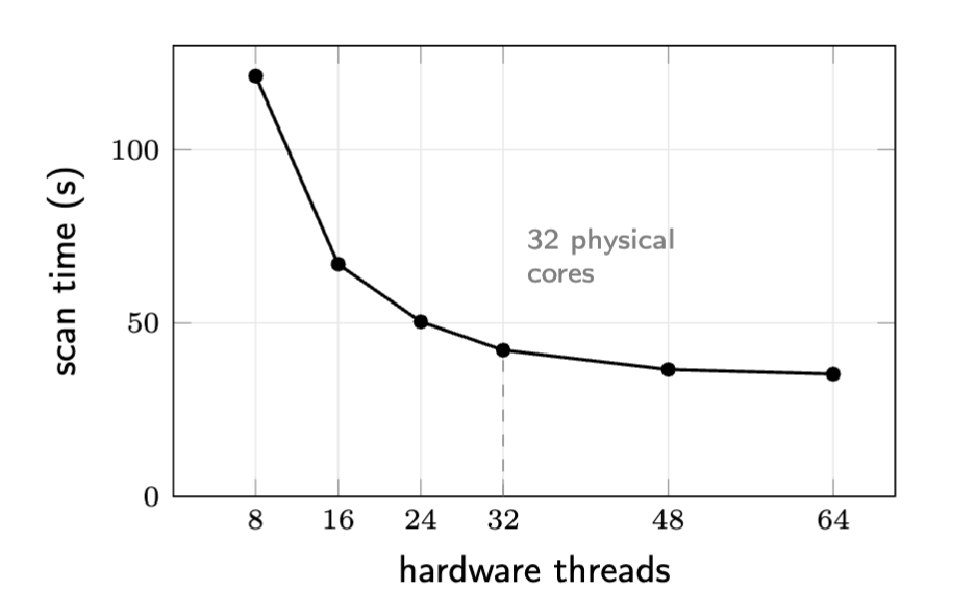
\includegraphics[width=0.55\linewidth,height=0.4\textheight,keepaspectratio]{figures/Figure_5}
\caption{Scaling of the fixed 400-item scan on platform P. Every configuration produces the same 11,005 findings. The horizontal axis is hardware threads, not physical cores: the platform has 32 cores, so the 48 and 64 points add simultaneous multithreading siblings rather than cores. Single runs.}
\label{fig:scaling-p}
\end{figure}

The curve of Figure~\ref{fig:scaling-p} flattens as the thread count approaches the physical core count, but its last two points cannot carry a saturation argument on their own. Once the 32 physical cores are occupied, the additional threads are SMT siblings whose contribution to a memory-bound workload is a fraction of a core's; a diminishing return there is the expected behaviour of the hardware and is not by itself evidence of a serial residue in the software. Distinguishing the two requires a platform that adds cores without adding siblings.

\begin{figure}[H]
\centering
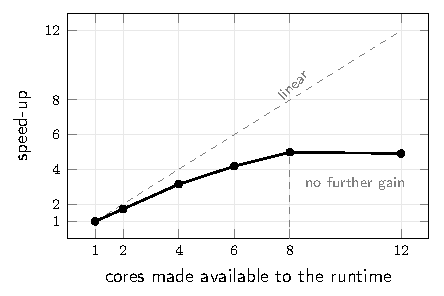
\includegraphics[width=0.55\linewidth,height=0.4\textheight,keepaspectratio]{figures/Figure_6}
\caption{Scaling of the fixed 400-item scan on platform A, which presents one hardware thread per core, so the abscissa varies cores and nothing else. Median of three runs per point. The speed-up reaches 4.99 at eight cores and does not improve at twelve.}
\label{fig:scaling-a}
\end{figure}

Platform A is such a platform: it reports one hardware thread per core, so varying the number of cores the runtime may use varies cores and nothing else. The measurement was repeated there, starting a separate engine instance for each setting with the runtime's processor count pinned and the worker pool set to match, three runs per point, with the production instance untouched throughout; Figure~\ref{fig:scaling-a} reports the result.

The curve stops rising at eight of the twelve available cores. The measured speed-ups are 1.71, 3.14, 4.18 and 4.99 at two, four, six and eight cores, and 4.91 at twelve---within the run-to-run spread of the eight-core point, so the last four cores contribute nothing measurable. Dispersion is small except at the single-core point, whose first run was some 44 s slower than its other two and whose inter-quartile range is correspondingly wide at 22.1 s; the index is constructed on first use, so that run carries a cost the others do not, and the median is reported for this reason.

This is a weaker result than the production-node curve appeared to give, and it is the one the placement argument should rest on. Amdahl's relation \cite{amdahl1967} implies a serial fraction of 8.6\% from the eight-core point, and the residue is serial by construction---the in-memory index is built once, the request planned once, the response serialised once at the end. But the same relation implies 13.1\% from the twelve-core point, and a genuine fixed serial section would imply the same fraction from both. The discrepancy indicates a second mechanism whose cost grows with the number of active workers, on this platform most plausibly the co-located store, which enrichment still consults after the decision phase. Platform A's one-thread-per-core property comes bundled with store co-location, and the two cannot be separated without a third machine. What can be said is bounded accordingly: on this hardware the parallel speed-up stops at eight cores, and whether a machine with a remote store would carry it further is not established here.

\paragraph{An invariant that did not hold.}
One anomaly is reported rather than smoothed, because pursuing it produced a result that bears on the system rather than only on the experiment. The finding set was identical within every point of the sweep but not across points: the one- and two-core points returned 216,861 findings against 216,828 at four cores and above. The sweep runs for about an hour against a corpus refreshed on a background schedule, so a feed update partway through was the natural explanation, and the count changing once rather than varying with worker count was consistent with it.

A controlled check was therefore run: the same workload submitted alternately at one and at twelve workers, with the engine's binary digest read immediately before and after every scan so that a rebuild during the test would invalidate it rather than corrupt it. Two observations were obtained under one unchanging engine, 64 seconds apart. At one worker the scan returned 216,841 findings and at twelve 216,861, with the threat count identical in both at 136,030---so the twenty-finding difference lies entirely in the cleared and undetermined buckets.

That result does not support the corpus-drift explanation, and is reported as not supporting it. A feed update in the intervening minute that added findings while leaving the threat count exactly unchanged would be a coincidence, whereas a difference in how a concurrently evaluated candidate set is ordered or tie-broken produces precisely this signature---and this system has met that failure before, when an incompletely ordered retrieval let the store break ties arbitrarily. The evidence is one pair rather than a replicated series, because repetition was prevented by the engine binary being rebuilt during the test twice, which the identity check caught and which is itself an instance of the hazard of Section~\ref{sec:measuring}. The claim is bounded accordingly: on the build measured, the invariant that every configuration produces the same findings does not hold across worker counts, the cause is not established, and the matter is open. Timings are unaffected either way---twenty findings in 216,861 cannot account for a factor of five---but parity across worker counts within the compiled engine, unlike the interpreted-versus-compiled parity of Section~\ref{sec:verdict-preservation}, was assumed rather than tested and is now known to deserve testing.

The consequence for placement follows directly. If the workload stops gaining beyond eight cores, throughput is not something a larger central machine can sell; a twelve-core appliance already sits past the point where this workload can use additional cores, and the 32-core node is provisioned well beyond it. What argues for the larger machine, if anything does, is the resource footprint of Section~\ref{sec:footprint} rather than the core count.

The utilisation figures are consistent with a workload that cannot occupy a whole machine. On the production node the end-to-end scan of Section~\ref{sec:e2e} held 21.9 of 32 cores busy on average (68\%) and 29.1 at peak (91\%); on the twelve-core appliance the 400-item scan accumulated 1,258 s of phase-attributed work in 164.5 s of wall time, an effective 7.6-fold overlap, or 64\% of the machine. Two platforms and two instrumentation methods give the same answer---the engine occupies about two thirds of whatever machine it is given---and the sweep identifies the residual third as the part that does not parallelise, whether because it is serial by construction or because the added workers contend for the store.

\subsection{The Model Runs Faster Without the Accelerator}
The remaining objection to edge placement is the neural component, which appears to require an accelerator and therefore a server. It does not. Exporting the tagger to a portable graph format \cite{onnx} required reimplementing the conditional-random-field decoding in the host language, since the decoder contains a data-dependent loop that does not export cleanly; the decoder is three small tensors and a deterministic search, so this was tractable, and decoding equivalence was verified over 300 real descriptions with identical label sequences from both paths.

The exported model on CPU runs at 4.0 ms per advisory against 8.3 ms for the GPU reference. At 8.8M parameters the arithmetic does not amortise kernel-launch overhead. This is not a general claim about neural inference; it is a claim about this model, and its consequence is specific: the appliance needs no accelerator, which removes the last hardware argument for centralisation.

\subsection{Resource Footprint}
\label{sec:footprint}
A deployment argument that reports no resource figures is an assertion, so the budget is stated in Table~\ref{tab:footprint}.

% Table 16: Resource footprint of the production node.
\begin{table}[htbp]
\centering
\caption{Resource footprint of the production node (P) during a production scan. Index load and resident size were also measured on the appliance (A), where the index loads in 25.8--29.0 s.}
\label{tab:footprint}
\footnotesize
\begin{tabular}{l r}
\hline
Quantity & Value \\
\hline
Engine: start-up to listening & $<$ 1 s \\
Engine: index load & 25.8--32.2 s \\
Engine: resident, index loaded & 1.35--1.55 GB \\
Engine: resident, prolonged idle & $\approx$4.04 GB \\
Engine: resident during scan, mean & 5.34 GB \\
Engine: resident during scan, peak & 8.40 GB \\
Engine: threads at peak & 42 \\
Service tier: resident & $\approx$70 MB \\
Service tier: processor during scan & 0.3--0.6\% \\
Store: resident (incl. shared buffers) & $\approx$4.01 GB \\
Database on disk & 2,370 MB \\
Feed working copy on disk & 4.0 GB \\
Model files on disk & 170 MB \\
Application image on disk & 210 MB \\
\hline
\end{tabular}
\end{table}


The memory profile has three tiers, as expected of a garbage-collected runtime: about 1.5 GB with the index freshly loaded, a working set near 4 GB after prolonged operation, and a transient peak of 8.4 GB during a scan arising from per-item candidate lists and decision structures. The peak recedes when the scan ends and sets the sizing rule: 16 GB is a floor and 32 GB comfortable. The service tier is negligible beside this---roughly 70 MB resident and under 1\% of a core---because the decision is taken in the engine while the tier only authenticates, plans, meters, caches and serialises. That asymmetry is a continuity property as well as a sizing one: the tier restarts without reloading the index, so a release of the request-handling path costs no scan capacity.

\subsection{Throughput}
Table~\ref{tab:throughput} reports aggregate service behaviour across the workloads of Section~\ref{sec:methodology}.

% Table 17: Measured end-to-end service performance.
\begin{table}[htbp]
\centering
\caption{Measured end-to-end service performance. All rows are platform A except the final row, which is the production node (P).}
\label{tab:throughput}
\footnotesize
\begin{tabular}{l r}
\hline
Scenario & Value \\
\hline
Cold scan, single item & 1.5--3.1 s \\
Cache hit & $\approx$12 ms \\
Same product, five versions & 8.2 s $\rightarrow$ 2.1 s (3.9$\times$) \\
29-item inventory, 20 duplicates & 9.9 s (0.34 s/item) \\
40-item request, cold then warm & 81.2 s $\rightarrow$ 10.2 s \\
300 items, cold cache & 188 s (1.6 items/s) \\
300 items, warm cache & 10.1 s (29.7 items/s) \\
1,443 items, production inventory & 368.1 s (3.9 items/s) \\
\hline
\end{tabular}
\end{table}


Aggregate rates conceal a wide per-item spread, and the spread rather than the mean is what an operator plans against: a product with thousands of candidate advisories costs several times a small application, so the mean reflects the composition of a particular estate rather than a property of the engine. Throughput is reported because it is what was measured end to end, but the statistic a NAC admission budget is written against is the per-item latency distribution, reported next. The ratio between a cache hit and a cold scan is roughly 130, which is why the concentration result of Section~\ref{sec:estate} matters operationally: the head items that dominate row counts are the ones that will be warm, while the singleton tail sets the floor on estate scan time and no cache size changes that.

\subsection{Per-Item Latency on the Interactive Path}
A posture decision is taken within a time budget, and a budget is written against a tail percentile rather than against an aggregate rate. The distribution was therefore measured directly, on the path that a synchronous single-endpoint check uses: 200 items drawn from the configuration workload in shuffled order, each submitted as its own request against a warm engine, one worker per request. Measuring inside a batch would have described queueing rather than the budget, because items in a batch overlap by design. Table~\ref{tab:latency} reports the result and Figure~\ref{fig:latency} the distribution behind it.

% Table 18: Per-item latency on the interactive single-item path.
\begin{table}[htb]
\centering
\caption{Per-item latency on the interactive single-item path (platform A, warm engine, $n = 200$ requests).}
\label{tab:latency}
\footnotesize
\begin{tabular}{l r}
\hline
Statistic & Latency \\
\hline
Minimum & 4.6 ms \\
25th percentile & 320 ms \\
Median & 765 ms \\
75th percentile & 1.16 s \\
Inter-quartile range & 838 ms \\
Mean & 888 ms \\
90th percentile & 1.71 s \\
95th percentile & 3.20 s \\
99th percentile & 3.69 s \\
Maximum & 3.89 s \\
\hline
\end{tabular}
\end{table}


\begin{figure}[!htb]
\centering
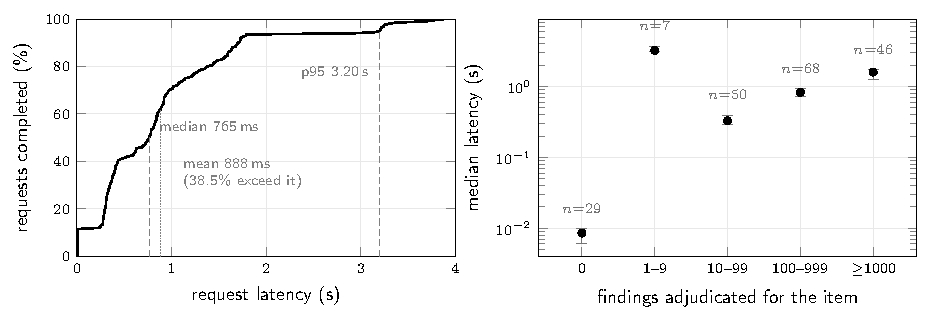
\includegraphics[width=0.85\linewidth,height=0.4\textheight,keepaspectratio]{figures/Figure_7}
\caption{Per-item latency on the interactive single-item path (platform A, warm engine, $n = 200$). (a) The measured distribution: the mean is exceeded by 38.5\% of requests, which is why an admission budget written against it is missed by more than one request in three. (b) Median latency per decade of adjudicated findings, with the bucket population above each point. Among the 164 items yielding ten or more findings the cost tracks candidate volume (Spearman's $\rho = 0.92$); the seven items yielding one to nine findings are the slowest class in the sample, because a generic product name obliges the engine to exhaust a wide candidate set before abstaining.}
\label{fig:latency}
\end{figure}

The distribution is what the throughput figures could not show. The tail is more than four times the median, and the mean is a poor budget: 38.5\% of requests exceed it and 6.0\% exceed three seconds, so a budget written against it would be missed by more than one request in three. That is the practical reason an aggregate rate cannot substitute for the distribution. The minimum of 4.6 ms is a cache hit, consistent with the $\approx$12 ms figure of Table~\ref{tab:throughput} and confirming that the two ends of this distribution are different code paths rather than the same path under load.

The slow tail is not random, and it has two distinct causes rather than one. Of the ten slowest requests in this sample, six are a single widely deployed document reader whose candidate advisory set is large, and the remaining four are generic single-word product names---the class Section~\ref{sec:estate} identifies as requiring vendor or platform context---for which the engine exhausts a wide candidate set before abstaining. The two mechanisms are separated in Figure~\ref{fig:latency}(b), which reports the median latency of each item against the number of findings the engine had to adjudicate for it.

Among the 164 items that produce ten or more findings the relationship is close to monotone---Spearman's $\rho = 0.92$---and the median rises through 328 ms, 828 ms and 1,598 ms across the three decades of finding count: cost on this path is governed by candidate volume. The exception is the seven items yielding between one and nine findings, with a median latency of 3,245 ms the slowest class in the sample. These are exactly the generic names---\texttt{Notes}, \texttt{Terminal}---that the engine cannot resolve to a product, and they are expensive for the opposite reason to the document reader: not because a large candidate set must be adjudicated, but because a large candidate set must be exhausted before the engine is entitled to abstain. Items that produce no finding at all are recognised as unmatched early and return in a median of 8.5 ms, so the expensive class is specifically the one that looks decidable and is not. That inverts an intuition the decision semantics invite: an item that cannot be decided is cheap to report but not cheap to reach, so abstention is paid for at the tail rather than saved at the median. An operator sizing an admission budget should provision for approximately four seconds per interactive item on this platform, and an estate-scale scan should be submitted in batches, where the same work overlaps.

\subsection{An End-to-End Estate Scan}
\label{sec:e2e}
The projections below apply a rate measured on a synthetic load test, and that input can be checked against a measurement of the same kind as the workload it is applied to. A production inventory of a further deployment was scanned end to end, with the operator's permission, using the queue-bypassing harness of Section~\ref{sec:measuring} so that the run is attributable to a named engine build.

The inventory comprises 6,129 application rows from 183 endpoints, reduced by the exporter to 1,443 scan items over 924 products---$\rho_{\text{item}} = 4.25$ and $\rho_{\text{group}} = 1.56$, both within the range of Table~\ref{tab:redundancy}. Its fan-out is likewise ordinary: a median of one endpoint per item, 68.1\% of items on exactly one endpoint, a maximum of 179, and the largest one percent of items covering 31.2\% of rows, with the head that Section~\ref{sec:estate} predicts made concrete as the inventory agent (179 endpoints), the endpoint security client (156) and an operating-system update package (140). That ordinariness is what makes it usable as a check on the projection.

The scan completed in 368.1 s and produced 32,497 threat findings over 513 items whose verdict was Threat, with 357 Safe, 410 NotFound and 163 Uncertain. The realised rate of 3.9 items per second against the projection's 1.6 makes the projection conservative by a factor of 2.4 on a workload 4.8 times larger than the load test it was derived from. A second, separately instrumented run completed in 268--273 s; the slower figure is reported because it is the run whose engine identity was recorded, for the reason given in Section~\ref{sec:measuring}. One qualification belongs with it: a single estate does not establish that the rate is workload-independent, only that the assumption did not fail where it could be tested.

\paragraph{The same estate on the appliance.}
Because the placement argument is about the appliance rather than the production node, the same inventory was subsequently scanned on platform A, three times, against the corpus snapshot current at that later date. The median was 468.8 s, with the three runs spanning 465.6--469.9 s---a coefficient of variation of 0.4\%---and all three produced an identical finding set. The comparison that matters is one of order rather than ratio: the twelve-core appliance completes a real 1,443-item estate in under eight minutes, against just over six on a node with 32 cores and a remote store. The two numbers are not directly comparable---different corpus snapshots, different verdict distributions, so no speed-up is computed from them---but they need not be: the difference between the appliance and the substantially larger central node is a matter of minutes on an operation the operator schedules daily. That is the empirical content of the placement claim, and it is weaker and more useful than a ratio would be.

\subsection{Projected Estate Scan Times}
What follows is the only part of this evaluation that is not measurement, and it is presented as a bracket rather than as a result. Table~\ref{tab:projected} applies the conservative 1.6 items/s rate to the workload figures of Section~\ref{sec:estate}; the operators of those estates consented to analysis of their exports but not to a scan against them, so no end-to-end figure for these eight estates exists or can be obtained without a further permission. A reader interested only in what was observed may take from this subsection its single robust conclusion---reducing before scheduling moves the pooled workload from 31 hours to under four---and read the table as the arithmetic behind it.

% Table 19: Estate scan time under three scheduling policies (projections).
\begin{table}[htbp]
\centering
\caption{Estate scan time under three scheduling policies, at the conservative 1.6 items/s load-test rate. These are projections: measured throughput applied to measured workload, not end-to-end estate measurements. Section~\ref{sec:e2e} reports a measured scan at 2.4 times this rate.}
\label{tab:projected}
\footnotesize
\begin{tabular}{l r r r r r}
\hline
 & \multicolumn{2}{c}{Workload} & \multicolumn{3}{c}{Projected time} \\
Estate & $R$ & $U$ & per row & per item & per group \\
\hline
E1 & 9,271 & 1,510 & 1.6 h & 16 min & 40 min \\
E3 & 81,368 & 4,741 & 14.1 h & 49 min & 1.9 h \\
E4 & 5,940 & 721 & 62 min & 8 min & 17 min \\
E5 & 13,120 & 2,377 & 2.3 h & 25 min & 60 min \\
E6 & 34,779 & 4,632 & 6.0 h & 48 min & 2.1 h \\
E7 & 5,417 & 1,629 & 56 min & 17 min & 48 min \\
E8 & 23,282 & 3,316 & 4.0 h & 35 min & 86 min \\
E9 & 6,311 & 1,635 & 66 min & 17 min & 41 min \\
\hline
Pooled & 179,488 & 20,561 & 31.2 h & 3.6 h & 8.9 h \\
\hline
\end{tabular}
\end{table}


The status of these numbers should be explicit. The per-row and per-item columns apply one measured rate to two workload definitions; their ratio is exactly $\rho_{\text{item}}$ and carries no assumption beyond the rate being workload-independent. The per-group column is different in kind: it is analytic, computed as $G \times c_{\text{prep}}$ from Table~\ref{tab:single-product}, and assumes no cache reuse whatever. That it exceeds the empirical per-item column is informative rather than embarrassing---the load test behind the 1.6 items/s rate contains repeated products, so the planner and the persistent extraction cache are both active during it, while the analytic column excludes both. The two bracket the truth, and an estate scan should be expected to land between them. The operationally relevant comparison remains the first two columns: reducing before scheduling turns a 31-hour pooled workload into a 3.6-hour one, and turns E3 from an overnight batch that does not fit a maintenance window into a task completing within one.

\subsection{Verdict Preservation}
\label{sec:verdict-preservation}
A system rewritten for speed is a system whose verdicts might have changed. Four checks guard against that, and all four are release gates rather than one-off experiments.

\textbf{Engine parity.} Run over the same 146-item production inventory, the compiled engine and the reference implementation both report 2,904 threats with identical advisory sets. Missed and extra threats are reported separately rather than as one difference count, because they mean different things operationally.

\textbf{Decoding equivalence.} The two conditional-random-field decoders produce identical label sequences over 300 real advisory descriptions---a stronger check than comparing aggregate accuracy, which can coincide while individual decodings differ.

\textbf{Index equivalence, self-enforced.} The in-memory index is correct only if it returns what the store's query would have returned. The engine checks this against itself at start-up over a sample of products drawn using the production query form, and declines to enable the index if any candidate is missing, the scan then proceeding over the store, slower and unchanged. Equivalence broke four times during development and the check caught each: a missing full-text branch that lost 1,421 candidates for one product; a filter that dropped advisories without structural rows, and with them 41\% of the corpus; stemming applied on one side only; and an incomplete sort order that cost determinism. The check itself failed once in the more dangerous direction, passing while real scans still missed 89 threats because it did not account for vendor---which is why its sample now uses the production query form.

\textbf{Restart recovery.} A sixteen-item job was terminated once seven items had been recorded; on restart the worker took up the remaining nine and no item was processed twice. The negative case---requeuing running after worker start---was found the same way and fixed by ordering rather than by locking.

Determinism is treated as a property to be tested rather than assumed, after an incomplete sort order let the store break ties arbitrarily and produce different results on identical input; failures of this kind are invisible to accuracy metrics computed from a single run. The four checks test it along one axis only, repeated runs of one configuration, and Section~\ref{sec:scaling} indicates a second axis is not covered: on the same build the finding set differed between one worker and twelve, in the cleared and undetermined buckets while the threat count held. Determinism across configurations is therefore an open question rather than an established property, and is stated here as such rather than among the guarantees. Beyond these checks, 498 automated tests cover schema validation, authentication, quota, version comparison, name normalisation and gate logic without requiring a database.

\section{Discussion}
\label{sec:discussion}

\textbf{Estate structure is a system parameter, and it is measurable.} The two reduction ratios determine what a scanner can achieve before any implementation choice is made, and they vary by a factor of five across the estates observed here. A deployment that measures them can predict its own scan time; one that does not is guessing. Reporting $\rho_{\text{item}}$ alongside throughput would be a useful convention in future work, since throughput alone does not determine estate scan time. The same measurement carries an operational corollary: the estate with the most uniform imaging was by a wide margin the cheapest to scan per endpoint, so consolidating software builds pays a security-operations dividend that is not usually counted.

\textbf{Inventory quality bounds assessment quality, and part of it is fixable at source.} Nearly half the live rows observed here cannot be assessed because they carry no version. This is not a limitation of any scanner and cannot be addressed downstream; it is a property of what the platform collects, which makes it among the cheapest improvements available to an operator. The second quality problem is not fixable at source in the same way: the rows that do carry a version carry it under a display name the standardised dictionary does not recognise---2.6\% resolve unassisted, 13.0\% under the most generous normalisation measured---so an assessment service must treat name reconciliation as its primary matching problem rather than as preprocessing before a lookup. The two findings pull in opposite directions for a tool builder: the ceiling is set upstream, and the work below it is harder than the standard pipeline assumes.

\textbf{Measure before parallelising.} Thread-level concurrency made the scanner slower, and the profile that appeared to show I/O wait was core contention against a co-located store. Where the database shares the scanner's cores the usual reasoning about client concurrency inverts, and the durable fix was to remove the store from the per-item path rather than to schedule around it.

\textbf{Saturation is a placement argument, and it cuts against large machines.} On the platform where cores can be varied without confounding them with hardware threads, the parallel speed-up stops improving at eight cores. The measured saturation point implies that the throughput a centralised deployment would be bought with does not exist to be bought: the same production estate completed in 468.8 s on the twelve-core appliance against 368.1 s on the 32-core node, and the deployed node is provisioned above the point where this workload can use its cores. The two remaining arguments for centralisation---accelerator availability and operational convenience---are removed by the CPU result and by the coupling to the access control platform respectively. That conclusion depends on having varied cores rather than threads: past the physical core count the added units are SMT siblings, whose small contribution to a memory-bound workload is expected behaviour of the hardware rather than evidence about the software, and any placement argument turning on where parallelism stops should say which of the two it varied---the distinction is easy to miss because the operating system reports both under one name.

\textbf{Small models may prefer the CPU.} At 8.8M parameters the tagger ran roughly twice as fast on CPU as on GPU, because kernel-launch overhead dominated the arithmetic. For network appliances this removes the accelerator from the bill of materials and from the driver-compatibility surface.

\textbf{Correctness properties must survive the deployment mechanisms.} The two subtlest defects encountered were not in the decision logic. One was a cache that did not invalidate on code change; the other was an unordered response that buried the most urgent finding on the fourteenth page. Both produced wrong operator outcomes without the decision logic itself being at fault---and the measurement apparatus was itself a third such defect, when a shared job queue made three consecutive experiments report a change that had not been deployed.

\section{Threats to Validity}
\label{sec:threats}

\textbf{Estate sample.} Eight predominantly Windows estates from one vendor's NAC deployments in one country is a convenience sample. They span a factor of thirty in row count and differ markedly in provisioning discipline, which gives some confidence that the qualitative findings---two-level redundancy, heavy-tailed fan-out, incomplete version coverage---are not artefacts of a single deployment, but the specific ratios should not be transferred to other populations without measurement, which is why the analysis scripts are released.

\textbf{Missing operating-system component.} The merge key omits the operating-system family the deployed exporter includes, because these exports carry no such join. The omission can only merge items the deployed system would separate, so reported redundancy is an upper bound; the effect should be small in single-platform estates and larger in mixed ones, and has not been measured.

\textbf{Projections are mostly not measurements.} Table~\ref{tab:projected} applies a measured throughput to a measured workload for the eight estates, whose exports were obtained under confidentiality terms that do not extend to running the scanner against them. Section~\ref{sec:e2e} reports the one end-to-end scan that was permitted, on a further deployment, confirming the projection's direction while showing it conservative. One such confirmation is not eight, and the remaining columns should still be read as brackets.

\textbf{Single-run timings remain the norm.} Timings are single runs except where a repetition is explicitly reported. Four measurements are repeated---the fixed 400-item workload over ten runs (Section~\ref{sec:repeatability}), the core-count sweep at three runs per point (Section~\ref{sec:scaling}), the end-to-end production inventory, and the index load---and the per-item latency distribution is taken over 200 requests. Everything else is a single observation: the engine comparison of Table~\ref{tab:engine}, the in-memory index comparison of Table~\ref{tab:index}, the phase decompositions, the CPU-versus-GPU inference comparison, and the cold and warm throughput figures. For those, no confidence intervals are given and no significance testing is performed. The repeated measurements place run-to-run variation at 2.4\% of the median on this workload and platform, which licenses reading the large factors those single runs report but would not license reading a difference of a few percent from them; no such difference is claimed. Removing this limitation requires no new apparatus, only re-runs: five runs per configuration for Table~\ref{tab:engine}, three per point for Figure~\ref{fig:scaling-p} with the physical-core boundary marked, a per-advisory distribution on both devices for the CPU--GPU comparison, the cold 300-item figure repeated with the cache cleared, and three production-node runs of the end-to-end inventory. Each should be reported as $n$, median and inter-quartile range rather than as a mean, since the distributions observed here are right-skewed.

\textbf{The latency distribution covers one path only.} The distribution of Section~\ref{sec:results} is measured on the interactive single-item path, which is the one an admission budget is written against. It is not the distribution of per-item cost inside a batch, where items overlap; obtaining that requires per-item timings within a batch, and that instrumentation has not been added. Estate-scale scans are submitted in batches, so the reported tail bounds the interactive case and does not describe the batched one.

\textbf{Two platforms, and one scaling claim.} Figures are labelled by platform and should not be transferred between them. The concurrency and index experiments were run on the twelve-core appliance, where the store shares the scanner's cores; that is the condition they investigate, but their magnitudes do not describe the production node, where the store is remote. Conversely the end-to-end scan and the resource footprint were taken on the production node. The scaling question is where the difference is load-bearing: the production node's upper points add hardware threads to already-occupied cores, so that curve alone cannot separate a serial residue in the software from the diminishing return of simultaneous multithreading. The claim about where parallelism stops therefore rests on the appliance sweep, which has one thread per core, and the production-node curve is corroboration on a differently shaped machine rather than its basis. Neither curve licenses extrapolation beyond the core counts measured.

\textbf{Verdict quality is out of scope here.} What is established is that the optimisation work did not change what the system decides, not that what it decides is right. Precision, recall, and abstention calibration are evaluated in a separate study, and the parity check of Section~\ref{sec:verdict-preservation} inherits whatever error the reference implementation has.

\textbf{Single-node deployment.} A single-node architecture is reported here. Multi-node deployments, in which several management platforms feed a shared corpus, raise cache-coherence and partitioning questions that did not arise here.

\section{Conclusion}
\label{sec:conclusion}
The objective was to compute per-asset vulnerability exposure for managed enterprise networks within an operational window, and the decisive properties proved to be those of the estates rather than of the scanner. Measurement of eight production estates comprising 2,525 endpoints and 336,918 live application records revealed redundancy at two levels---collapsing identical product--version pairs removes 88.5\% of the workload, and grouping the remaining items by product reduces repeated product-level preparation operations by a further 34.7\% while retaining a separate decision for every version---distributed with a heavy tail in which the largest one percent of items covers up to half of all rows while roughly half of all items appear on a single endpoint. Two further properties bound what any method can achieve on this input: 46.7\% of live rows carry no version and are therefore unassessable, and the canonical route from a display string to a standardised product identifier resolves only 2.6\% of product strings unassisted and 13.0\% under the most generous normalisation measured. Normalisation and full-text retrieval are therefore the primary matching path rather than a fallback to it, and both limits are properties of the inventory rather than of any assessment method.

Designed around these properties, the service reduces before scheduling, shares version-invariant preparation without merging versions, and caches across scans rather than within them. Its decision engine achieves real concurrency on commodity cores: on the controlled 24-product workload it ran 9.6 times faster than the single-threaded reference implementation it replaced, and on a 146-item production inventory the two implementations produced identical verdicts---a parity result rather than an accuracy one, since verdict quality is evaluated separately (Section~\ref{sec:threats}). Moving candidate retrieval into memory took the store off the per-item path and made that placement possible; the parallel speed-up stops well below the core count a centralised deployment would provide, so centralisation buys throughput that does not exist; and the sequence tagger runs faster on CPU than on GPU, removing the accelerator from the appliance. A production inventory comprising 6,129 rows from 183 endpoints was reduced to 1,443 assessable items and scanned end to end in 368 seconds. These results place the computation inside the managed network, alongside the platform that produces the inventory, so that a document enumerating an organisation's attack surface never leaves the network it describes. The measurements that would most improve the evaluation are an end-to-end scan of each of the eight estates and the effect of provisioning discipline across a larger estate population; both are field studies, and both would sharpen figures that can currently only be bracketed.

\section*{Author Contributions}
\textbf{Ramazan Kocaoğlu:} Supervision, Conceptualization, Methodology, Validation, Writing -- review \& editing. \textbf{Basma Bakırcı:} Conceptualization, Methodology, Software, Investigation, Data curation, Formal analysis, Validation, Visualization, Writing -- original draft.

\section*{Funding}
This research did not receive any specific grant from funding agencies in the public, commercial, or not-for-profit sectors.

\section*{Competing Interests}
The authors declare that they have no known competing financial interests or personal relationships that could have appeared to influence the work reported in this paper.

\section*{Related Submission}
A companion manuscript by the same authors, concerning the decision-quality and data-quality properties of the same platform, is under review elsewhere. The two papers report disjoint contributions and share no results; the relationship is declared here so that the editors of both venues can assess it. In accordance with PeerJ policy, this manuscript-under-review is disclosed in prose and is not cited as a bibliography entry.

\section*{Ethics and Data Handling}
The inventory exports were obtained during integration projects with the consent of the organisations that own them; the end-to-end scan of Section~\ref{sec:e2e} was performed with the operator's separate permission to scan as well as to analyse. The exports identify endpoints by an opaque numeric identifier internal to the management platform, carrying no hostname, user, address or location, and no organisation is named or identifiable from the figures reported: estates carry arbitrary labels. Access was limited to the authors and the records were analysed on infrastructure operated by the organisations themselves rather than copied to a third party. What is reported throughout is derived aggregate statistics, and no individual record is reproduced except where a product name is quoted as a lexical example, which names commercial software rather than a customer. No personal data within the meaning of applicable data protection law was processed, and the study accordingly did not require review by an ethics committee; no approval number is claimed.

\section*{Data Availability}
The underlying customer inventories cannot be released because of confidentiality restrictions: they enumerate the complete software estate of identifiable organisations, which is precisely the document Section~\ref{sec:background} argues should not leave the network that produces it. Analysis scripts and derived non-identifying aggregate statistics supporting the Section~\ref{sec:estate} estate-structure study are provided as supplemental files with this submission. Those scripts regenerate every figure in Section~\ref{sec:estate} from an export in the platform's native format, so the analysis is reproducible by any operator of a comparable deployment against their own data. The proprietary assessment engine, service tier, and trained model weights cannot be released. See \texttt{DATA\_AVAILABILITY.md} and \texttt{CODE\_AVAILABILITY.md} in the supplemental files for the full public/restricted split.

\section*{Declaration of Generative AI Use}
During the preparation of this work the authors used Claude Code (Anthropic; Claude Sonnet 5 model; \url{https://claude.com/claude-code}), a generative AI coding assistant, for language editing and \LaTeX{} formatting assistance. The authors reviewed and edited the resulting text and take full responsibility for the content. Generative AI was not used for experimental design, data analysis, or the drawing of scientific conclusions, and no AI system is listed as an author.

\section*{Acknowledgements}
The authors thank the network operations teams who permitted analysis of their inventory exports, and the engineering staff whose production incidents are reported here as measurements. Basma Bakırcı acknowledges infrastructure and operational support from Rakort Bilgi Teknoloji A.Ş., Ankara, Turkey. Generative AI (Claude Code, Anthropic; Claude Sonnet 5) was used for general language editing and \LaTeX{} formatting assistance during manuscript preparation; see the Declaration of Generative AI Use above for the full disclosure.

\bibliography{references}

\end{document}
